
%
%	Comparison of secondary interaction models
%

\section{Comparison of secondary interaction models}\label{Sec_Model}
\Headerfooter{Comparison of secondary interaction models}
\vs\hs
In Ref.~\cite{2014Abe,2019Abe}, it was found that agreements of the secondary interaction model based on BERT remain poor and result in significant systematic uncertainty as described in Section~\ref{Subsec_MeasurementsNCQE}.
Therefore, I compare the observed data with the other secondary interaction models using the newly developed Geant4-based SK detector simulation.
Here, we use three secondary interaction models: BERT, BIC, and INCL++.
Before showing the results of comparing the observed data with these models, features of each model are described in Section~\ref{Subsec_Features}.





\subsection{Features of secondary interaction models}\label{Subsec_Features}
\vs\hs
Here, we confirmed some MC true information such as the number of neutrons, the number of gamma-rays, and energy of gamma-rays, using 500 years of atmospheric neutrino NCQE events in the SK fiducial volume.
Figure~\ref{neutron_Logz_Pro_NumSec_ncqe} shows the number of generated neutrons per process after primary interactions (see Figure~\ref{Introd_NCQE_PriSec}).
In this figure, others include inelastic scattering reactions by the long-lived neutral kaon (${\rm K}^{0}_{\rm L}$), $^{2}{\rm H}$, $^{3}{\rm H}$, and $^{3}{\rm He}$ and electron-nuclear interactions.
From this figure, we can confirm that most of neutrons are generated by neutron inelastic scattering reactions.
%The number of neutrons generated by each process is summarized in Table~\ref{tab:neutron_process}.
The number of neutrons generated by each process is summarized in top of Table~\ref{tab:pre_gamma}.
From this table, we can confirm that the number of neutrons generated by neutron inelastic scattering reactions is largely different among secondary interaction models.
The number of neutrons is largest in BERT while smallest in INCL++.\\
\hs
Figure~\ref{neutron_Logy_NumSec}, Figure~\ref{neutron_Logy_Num}, and Figure~\ref{neutron_Logy_NumCap} shows the number of neutrons generated after primary interactions, the total number of neutrons (sum of neutrons generated by primary interactions (hereafter referred to as ``primary neutrons'') and neutrons generated after primary interactions), and the number of neutron captures, respectively.
From these figures, we can confirm that more neutrons are generated and captured in BERT than other two models.
%The number of neutrons and neutron captures are summarized in Table~\ref{tab:neutron}.
The total number of neutrons and neutron captures are summarized in center of Table~\ref{tab:pre_gamma}.
In this table, the number of primary neutrons is common among secondary interaction models (see Figure~\ref{neutronNumPri}).
Moreover, the number of neutron captures is smaller than the total number of neutrons.
The reason is that two stable nuclei are generated by neutron inelastic scattering reaction with oxygen nucleus.
For example, the following reaction is occurred,
\begin{eqnarray}
	{\rm n}\,+\,^{16}{\rm O}\,\to\,^{4}{\rm He}\,+\,^{13}{\rm C}.
\end{eqnarray}
Since $^{4}{\rm He}$ ($\alpha$) and $^{13}{\rm C}$ are stable, the total number of neutrons decreases when this reaction occurs.

\clearpage

%\begin{table}[H]
%	\centering
%	\caption[The number of neutrons generated by each process]{
%	The number of neutrons generated by each process.
%	}\label{tab:neutron_process}
%	\vs
%	\begin{tabular}{lrrr} \hline \hline
%		NCQE (383,284~events)                      &    BERT &     BIC &  INCL++ \\ \hline
%		neutron inelastic scattering               & 178,029 & 124,582 & 107,027 \\
%		proton inelastic scattering                &  36,295 &  39,112 &  34,040 \\
%		$\pi^{+}$ inelastic scattering             &     349 &     297 &     285 \\
%		$\pi^{-}$ inelastic scattering             &     638 &     785 &     722 \\
%		$\mu^{-}$ capture                          &      10 &      15 &      12 \\
%		$\pi^{-}$ capture                          &   4,221 &   4,548 &   4,693 \\
%		gamma-nuclear interaction                  &      64 &      61 &      61 \\
%		others                                     &     196 &      45 &   2,164 \\ \hline
%		The number of generated neutrons           & 219,802 & 169,445 & 149,004 \\ \hline
%		The number of generated neutrons per event &  0.5735 &  0.4421 &  0.3888 \\ \hline \hline
%	\end{tabular}
%\end{table}

\begin{figure}[p]
	\centering
	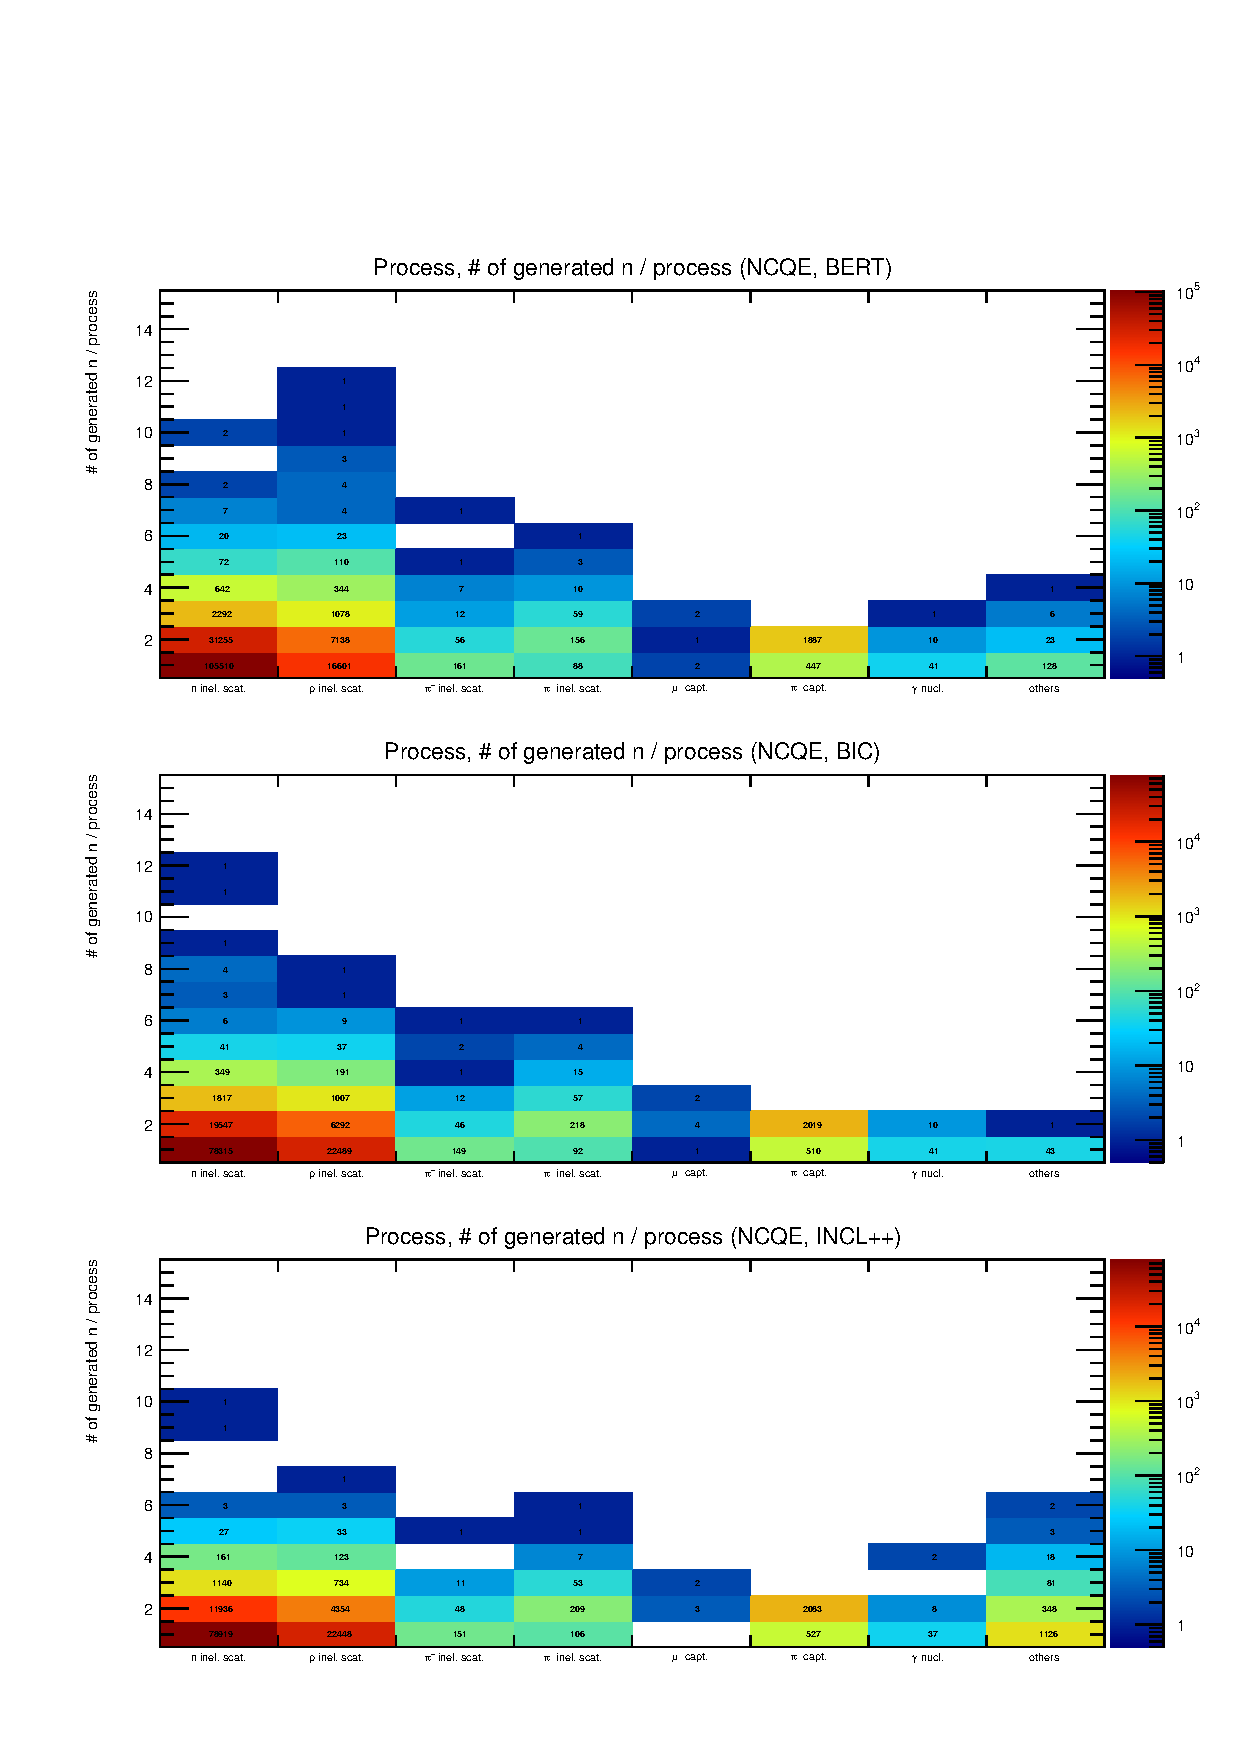
\includegraphics[width=15cm]{PDF/Secondary/Comparison/onlyNCQE_neutron/pdf2/Logz_Pro_NumSec_ncqe}
	\caption[The number of generated neutrons per process after primary interactions]{
	The number of generated neutrons per process after primary interactions.
	Top, center, and bottom figure shows the case of BERT, BIC, and INCL++, respectively.
	Horizontal axis shows processes that generated neutrons (neutron inelastic scattering, proton inelastic scattering, $\pi^{+}$ inelastic scattering, $\pi^{-}$ inelastic scattering, $\mu^{-}$ capture, $\pi^{-}$ capture, gamma-nuclear interaction, and others).
	}\label{neutron_Logz_Pro_NumSec_ncqe}
\end{figure}

\begin{figure}[p]
	\centering
	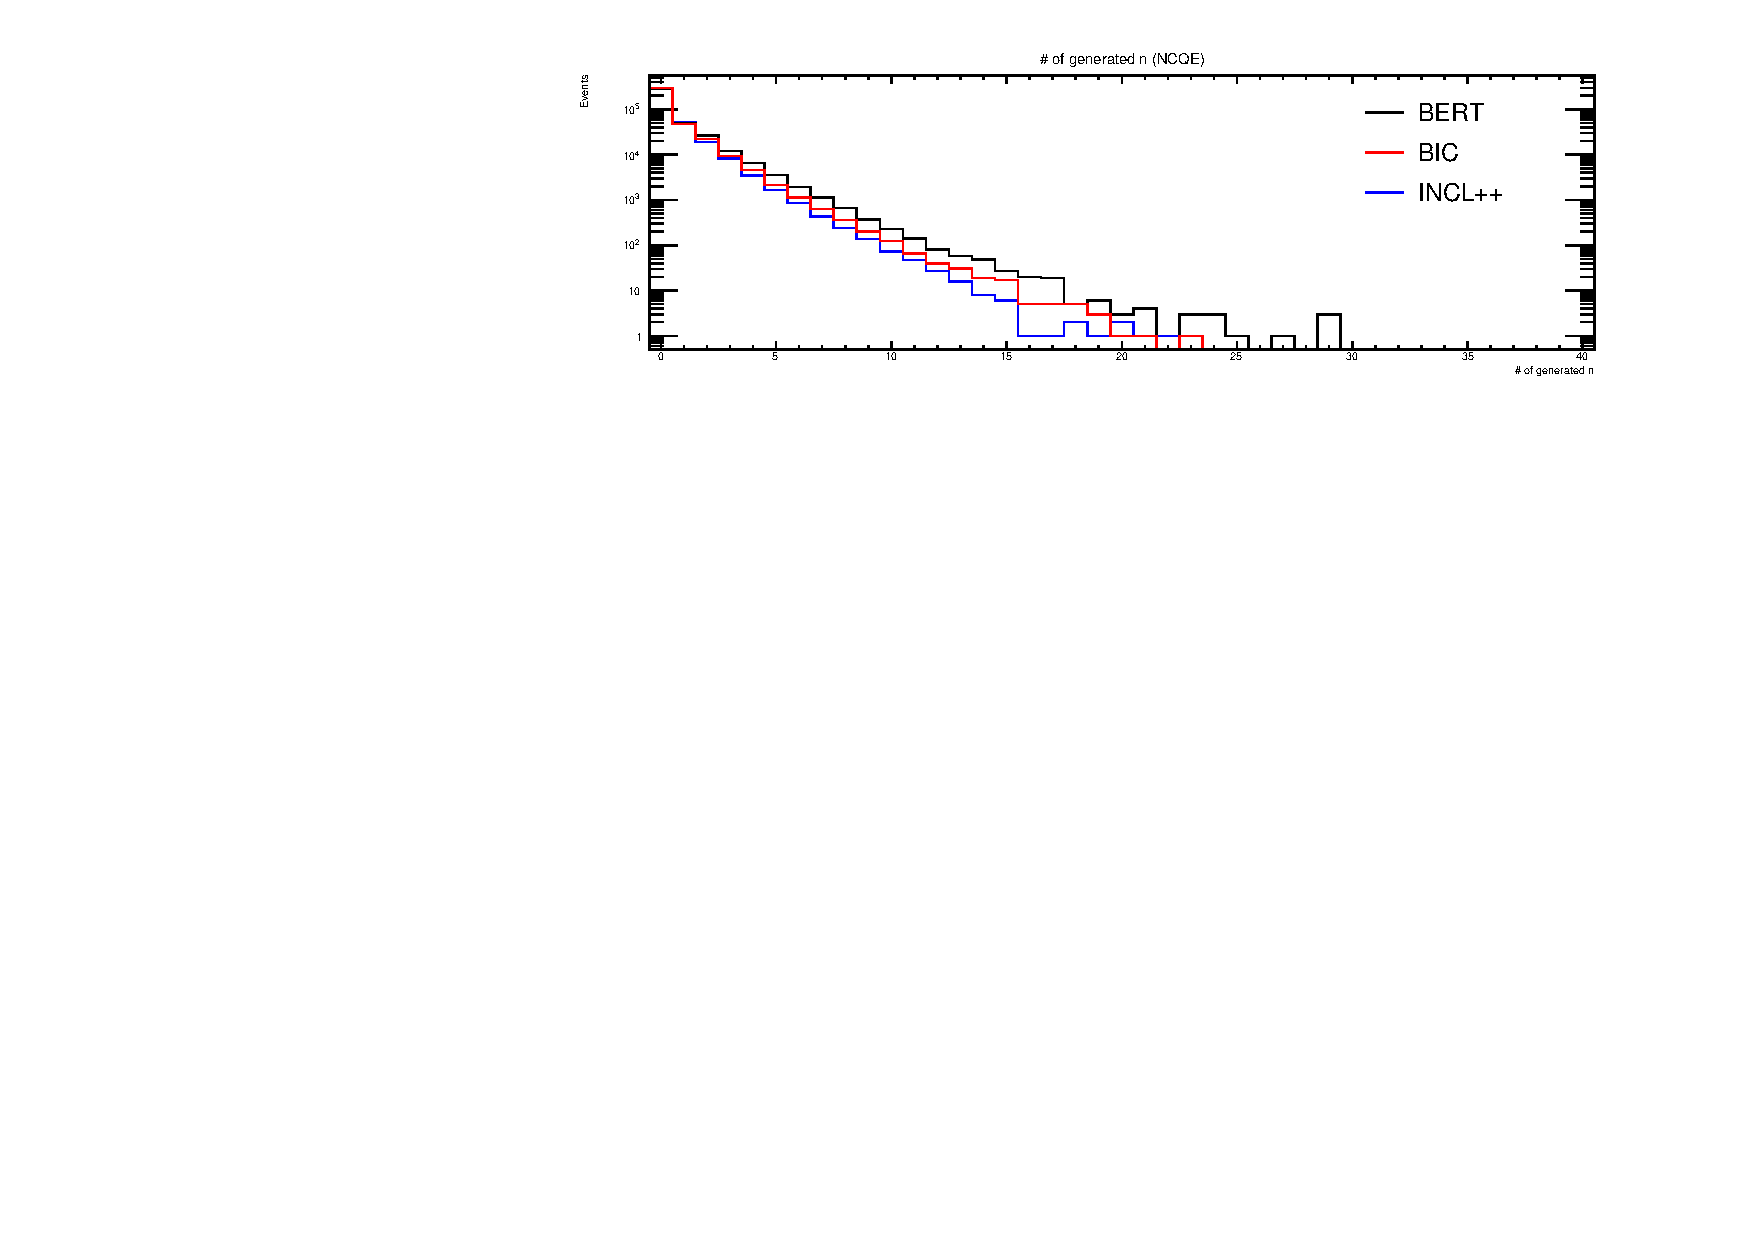
\includegraphics[width=16cm]{PDF/Secondary/Comparison/onlyNCQE_neutron/pdf1/Logy_NumSec}
	\caption[The number of neutrons generated after primary interactions]{
	The number of neutrons generated after primary interactions.
	Black, red, and blue line shows the case of BERT, BIC, and INCL++, respectively.
	}\label{neutron_Logy_NumSec}
\end{figure}

\begin{figure}[p]
	\centering
	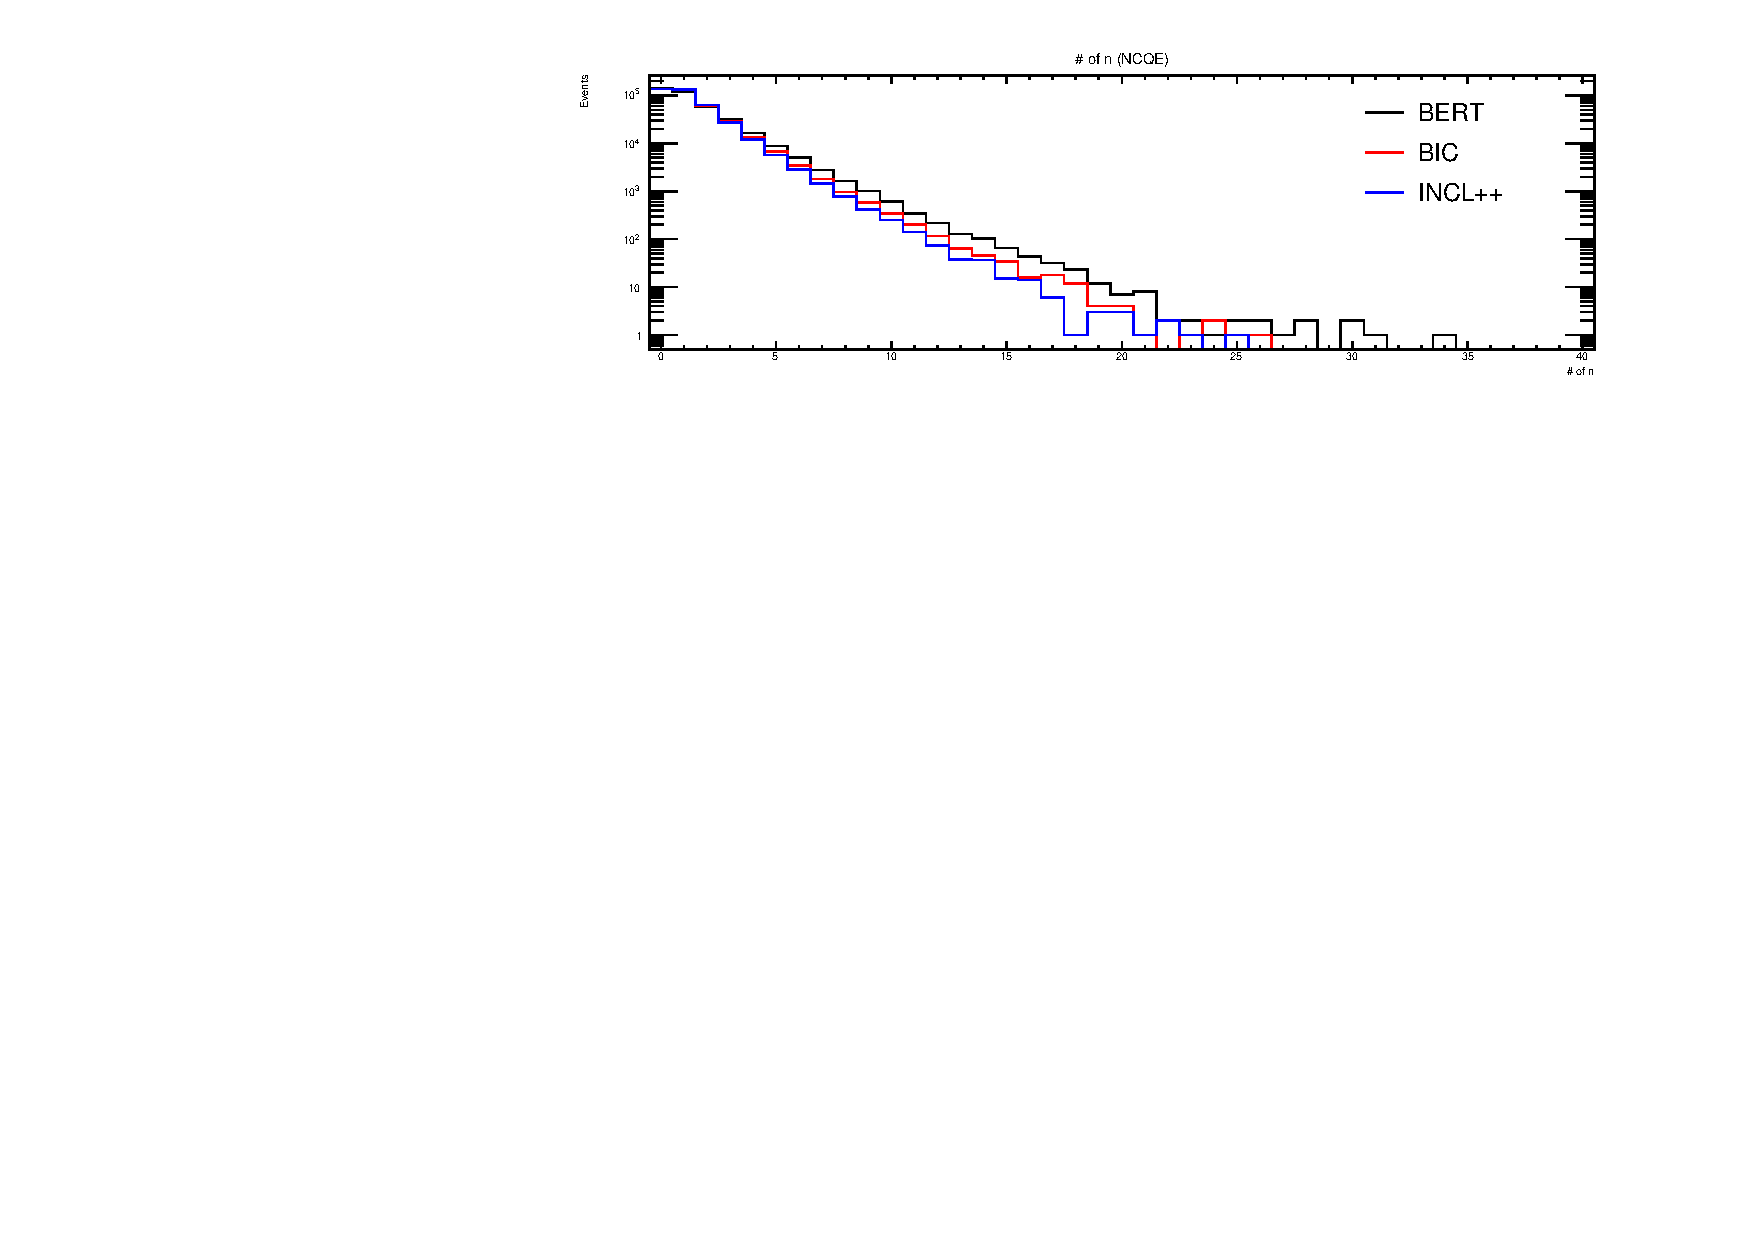
\includegraphics[width=16cm]{PDF/Secondary/Comparison/onlyNCQE_neutron/pdf1/Logy_Num}
	\caption[The total number of neutrons]{
	The total number of neutrons.
	Black, red, and blue line shows the case of BERT, BIC, and INCL++, respectively.
	}\label{neutron_Logy_Num}
\end{figure}

\begin{figure}[p]
	\centering
	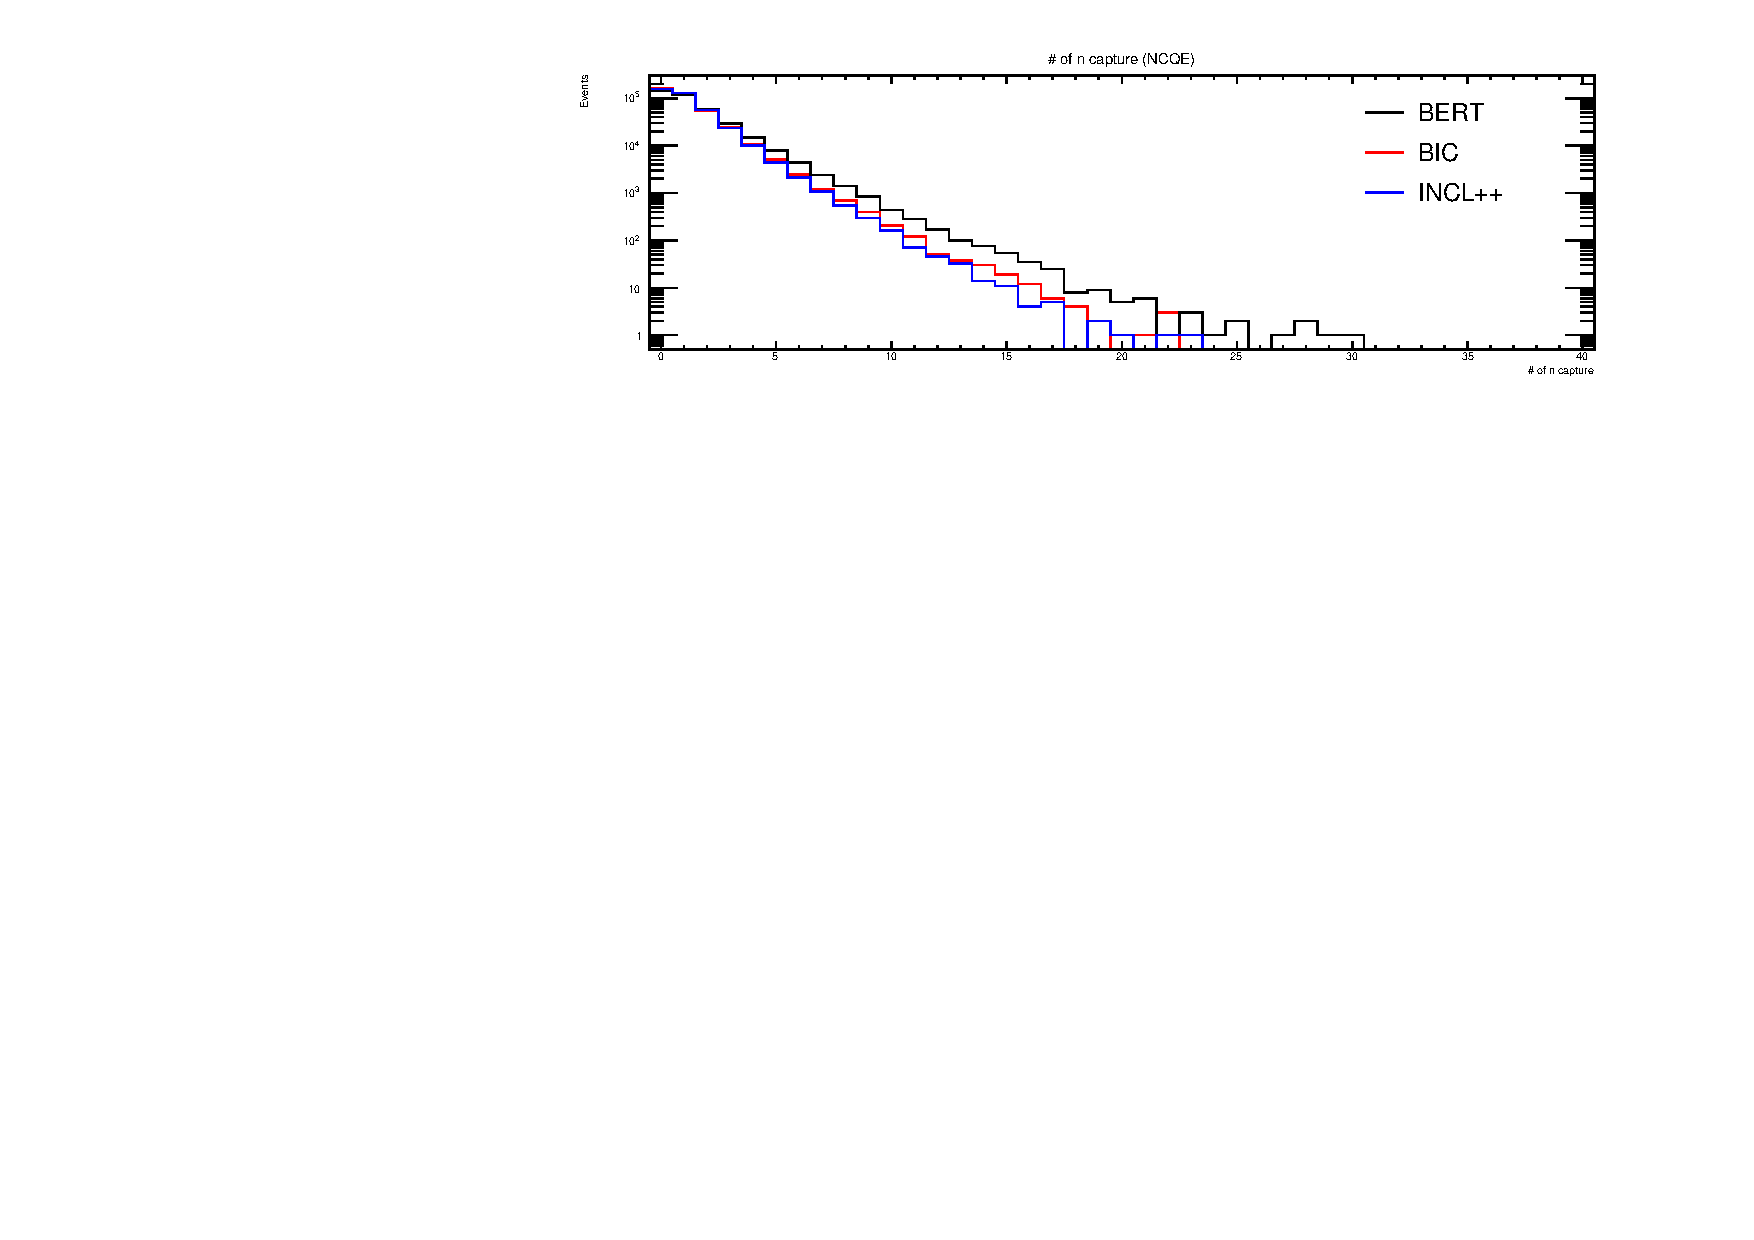
\includegraphics[width=16cm]{PDF/Secondary/Comparison/onlyNCQE_neutron/pdf1/Logy_NumCap}
	\caption[The number of neutron captures]{
	The number of neutron captures.
	Black, red, and blue line shows the case of BERT, BIC, and INCL++, respectively.
	}\label{neutron_Logy_NumCap}
\end{figure}

%\begin{table}[H]
%	\centering
%	\caption[The total number of neutrons and neutron captures]{
%	The total number of neutrons and neutron captures.
%	The number of primary neutrons is common among secondary interaction models.
%	}\label{tab:neutron}
%	\vs
%	\begin{tabular}{lrrr} \hline \hline
%		NCQE (383,284~events)                      &    BERT &     BIC &  INCL++ \\ \hline
%		The number of primary neutrons             & 310,835 & 310,835 & 310,835 \\
%		The number of generated neutrons           & 219,802 & 169,445 & 149,004 \\
%		The total number of neutrons               & 530,637 & 480,280 & 459,839 \\
%		The number of neutron captures             & 495,346 & 411,087 & 405,483 \\ \hline
%		The number of primary neutrons per event   &  0.8110 &  0.8110 &  0.8110 \\
%		The number of generated neutrons per event &  0.5735 &  0.4421 &  0.3888 \\
%		The total number of neutrons per event     &  1.3844 &  1.2531 &  1.1997 \\
%		The number of neutron captures per event   &  1.2924 &  1.0725 &  1.0579 \\ \hline \hline
%	\end{tabular}
%\end{table}

\clearpage

\hs
Next, we will focus on gamma-rays generated by neutron inelastic scattering reactions.
Figure~\ref{neutron_Logy_NumIne} shows the number of neutron inelastic scattering reactions.
The number of neutron inelastic scattering reactions is larger in BERT than other two models but not so different, and this trend is similar to that of Figure~\ref{neutron_Logy_NumSec}, Figure~\ref{neutron_Logy_Num}, and Figure~\ref{neutron_Logy_NumCap}.
However, the number of generated gamma-rays per neutron inelastic scattering reaction is largely different among secondary interaction models.
In Figure~\ref{gamma_NumSecIne}, the number of generated gamma-rays per neutron inelastic scattering reaction is similar between BIC and INCL++.
While, in BERT, it is apparently larger than other two models.
As a result, the number of gamma-rays generated by neutron inelastic scattering reactions is largely different between BERT and other two models, as shown in Figure~\ref{gamma_Logy_NumSec}.
Moreover, in BERT, events that the number of gamma-rays generated by neutron inelastic scattering reactions is one is small.
Energy of gamma-rays generated by neutron inelastic scattering reactions is also largely different.
In Figure~\ref{gamma_Logy_EneSec}, BERT has many continuous components in addition to peak structures of de-excitation gamma-rays, compared to other two models.
Furthermore, in Figure~\ref{gamma_Logy_TotEneSec}, total energy of gamma-rays generated by neutron inelastic scattering reactions, which is related to $E_{\rm vis}$, is larger in BERT than other two models.
%Information about the number of gamma-rays is summarized in Table~\ref{tab:gamma}.
Information about the number of gamma-rays is summarized in bottom of Table~\ref{tab:pre_gamma}.
In this table, the number of primary gamma-rays is common among secondary interaction models (see Figure~\ref{gammaNumPri}).
Moreover, the number of gamma-rays generated by neutron inelastic scattering reactions in BERT is more than twice as much as that in BIC and INCL++.

\begin{figure}[H]
	\centering
	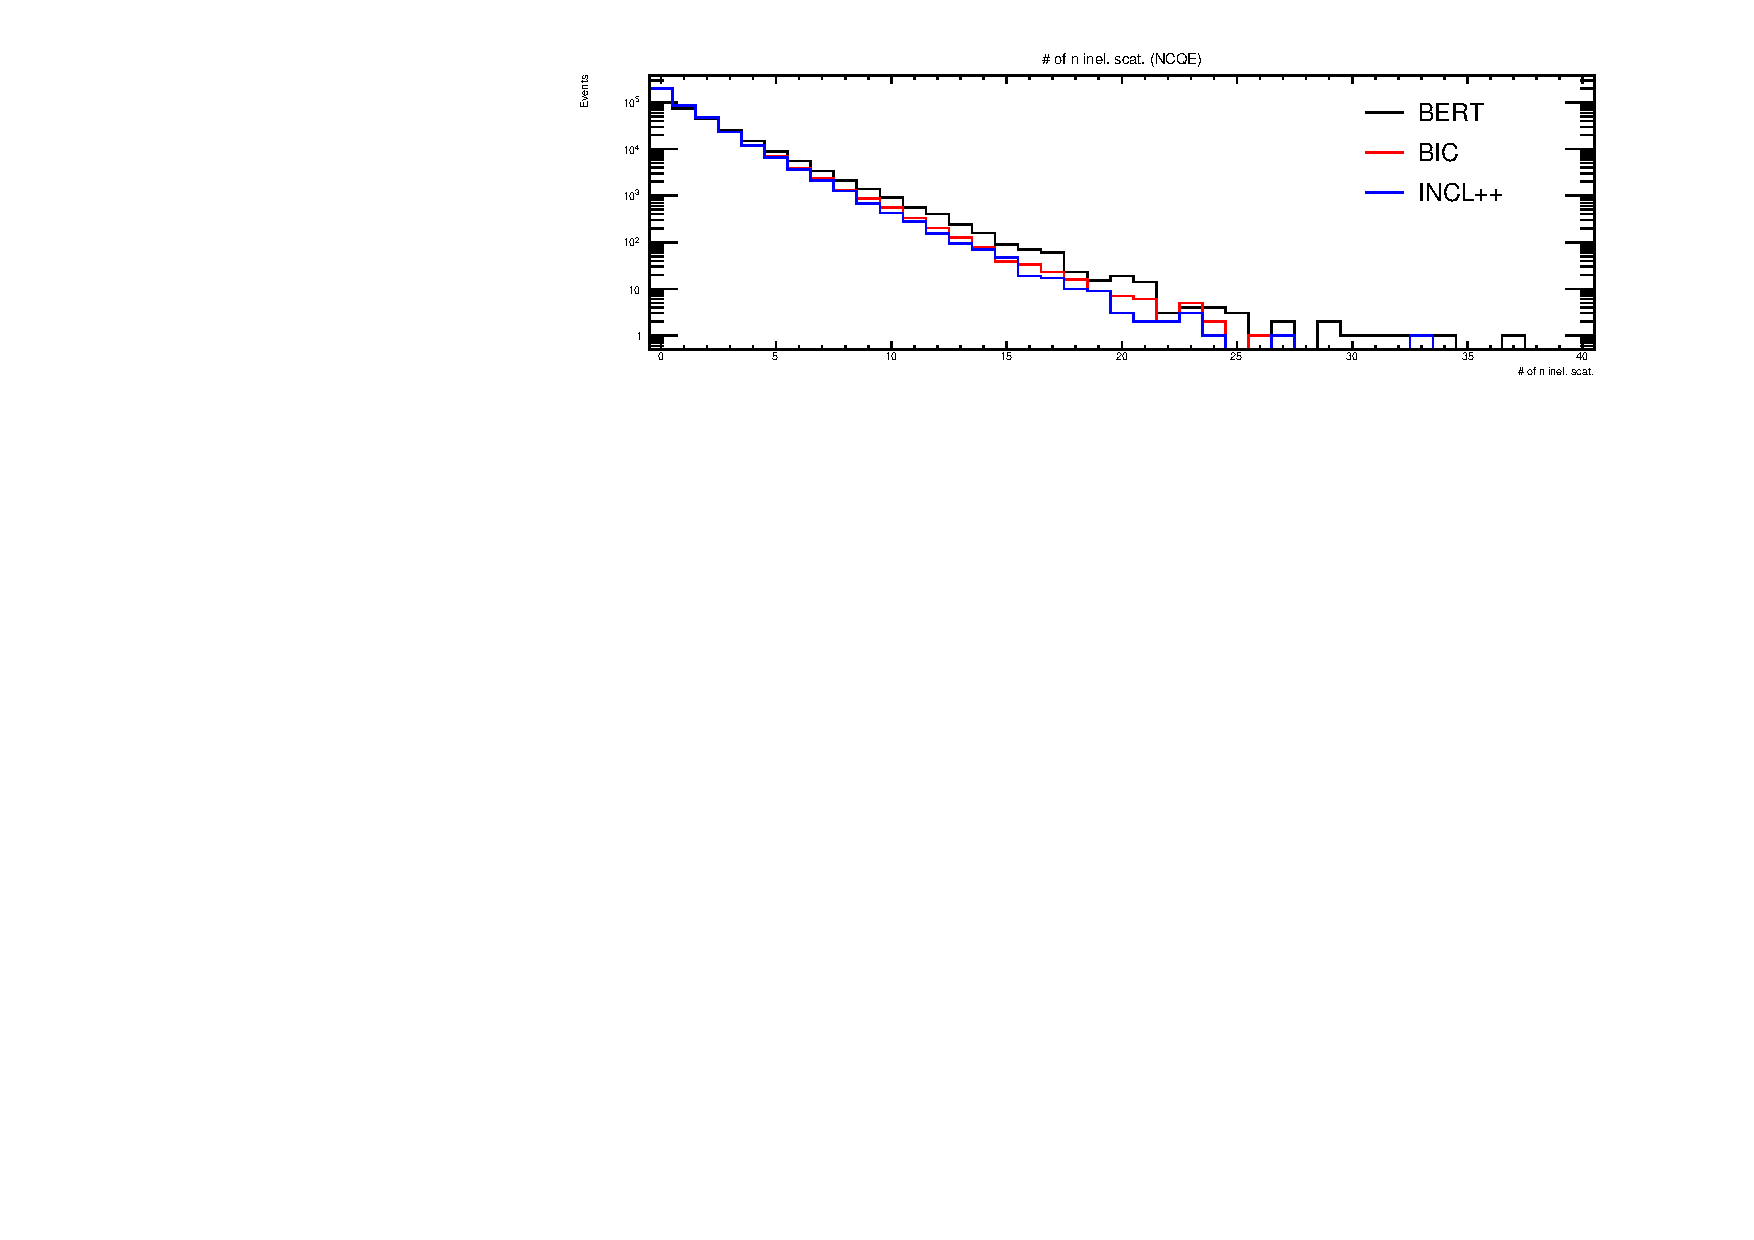
\includegraphics[width=16cm]{PDF/Secondary/Comparison/onlyNCQE_neutron/pdf1/Logy_NumIne}
	\caption[The number of neutron inelastic scattering reactions]{
	The number of neutron inelastic scattering reactions.
	Black, red, and blue line shows the case of BERT, BIC, and INCL++, respectively.
	}\label{neutron_Logy_NumIne}
\end{figure}

\begin{figure}[H]
	\centering
	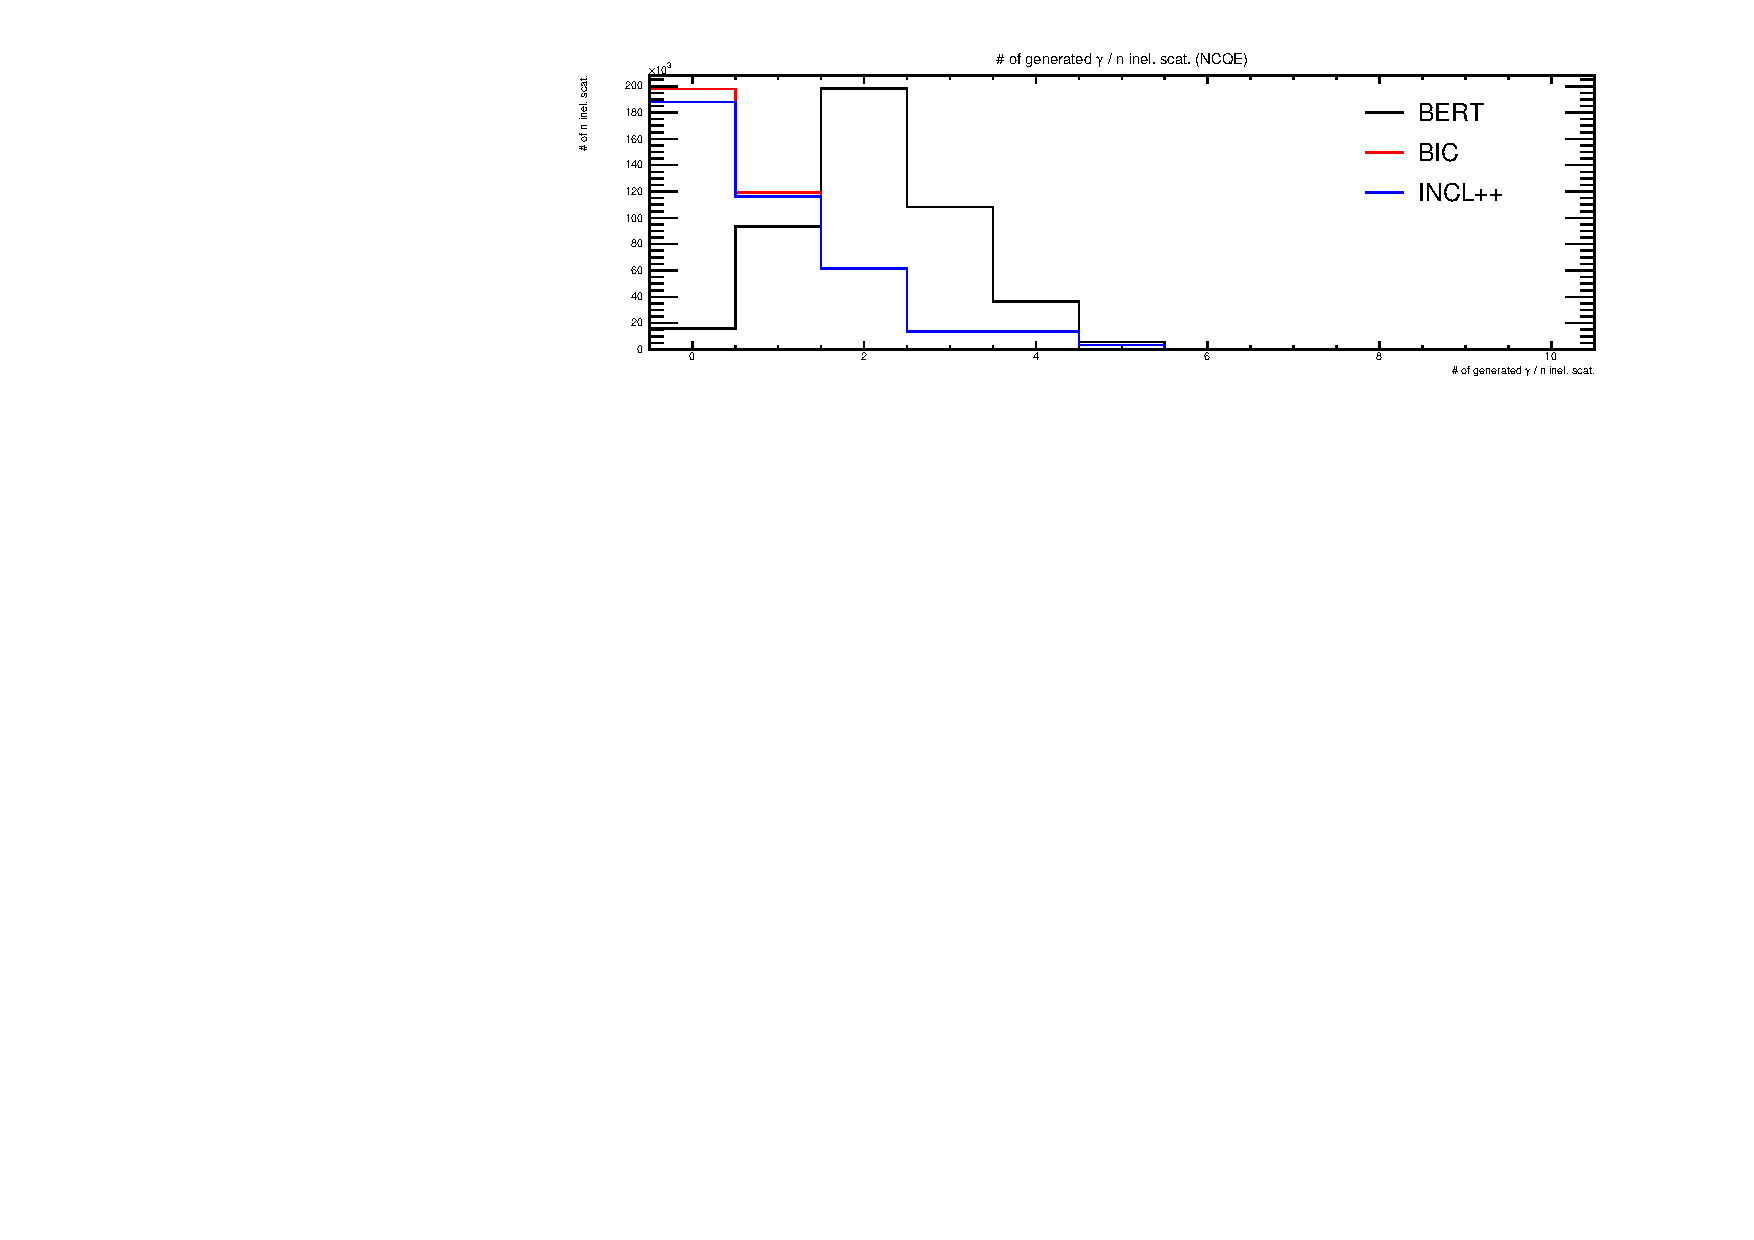
\includegraphics[width=16cm]{PDF/Secondary/Comparison/onlyNCQE_gamma/pdf1/NumSecIne}
	\caption[The number of generated gamma-rays per neutron inelastic scattering reaction]{
	The number of generated gamma-rays per neutron inelastic scattering reaction.
	Black, red, and blue line shows the case of BERT, BIC, and INCL++, respectively.
	}\label{gamma_NumSecIne}
\end{figure}

\begin{figure}[p]
	\centering
	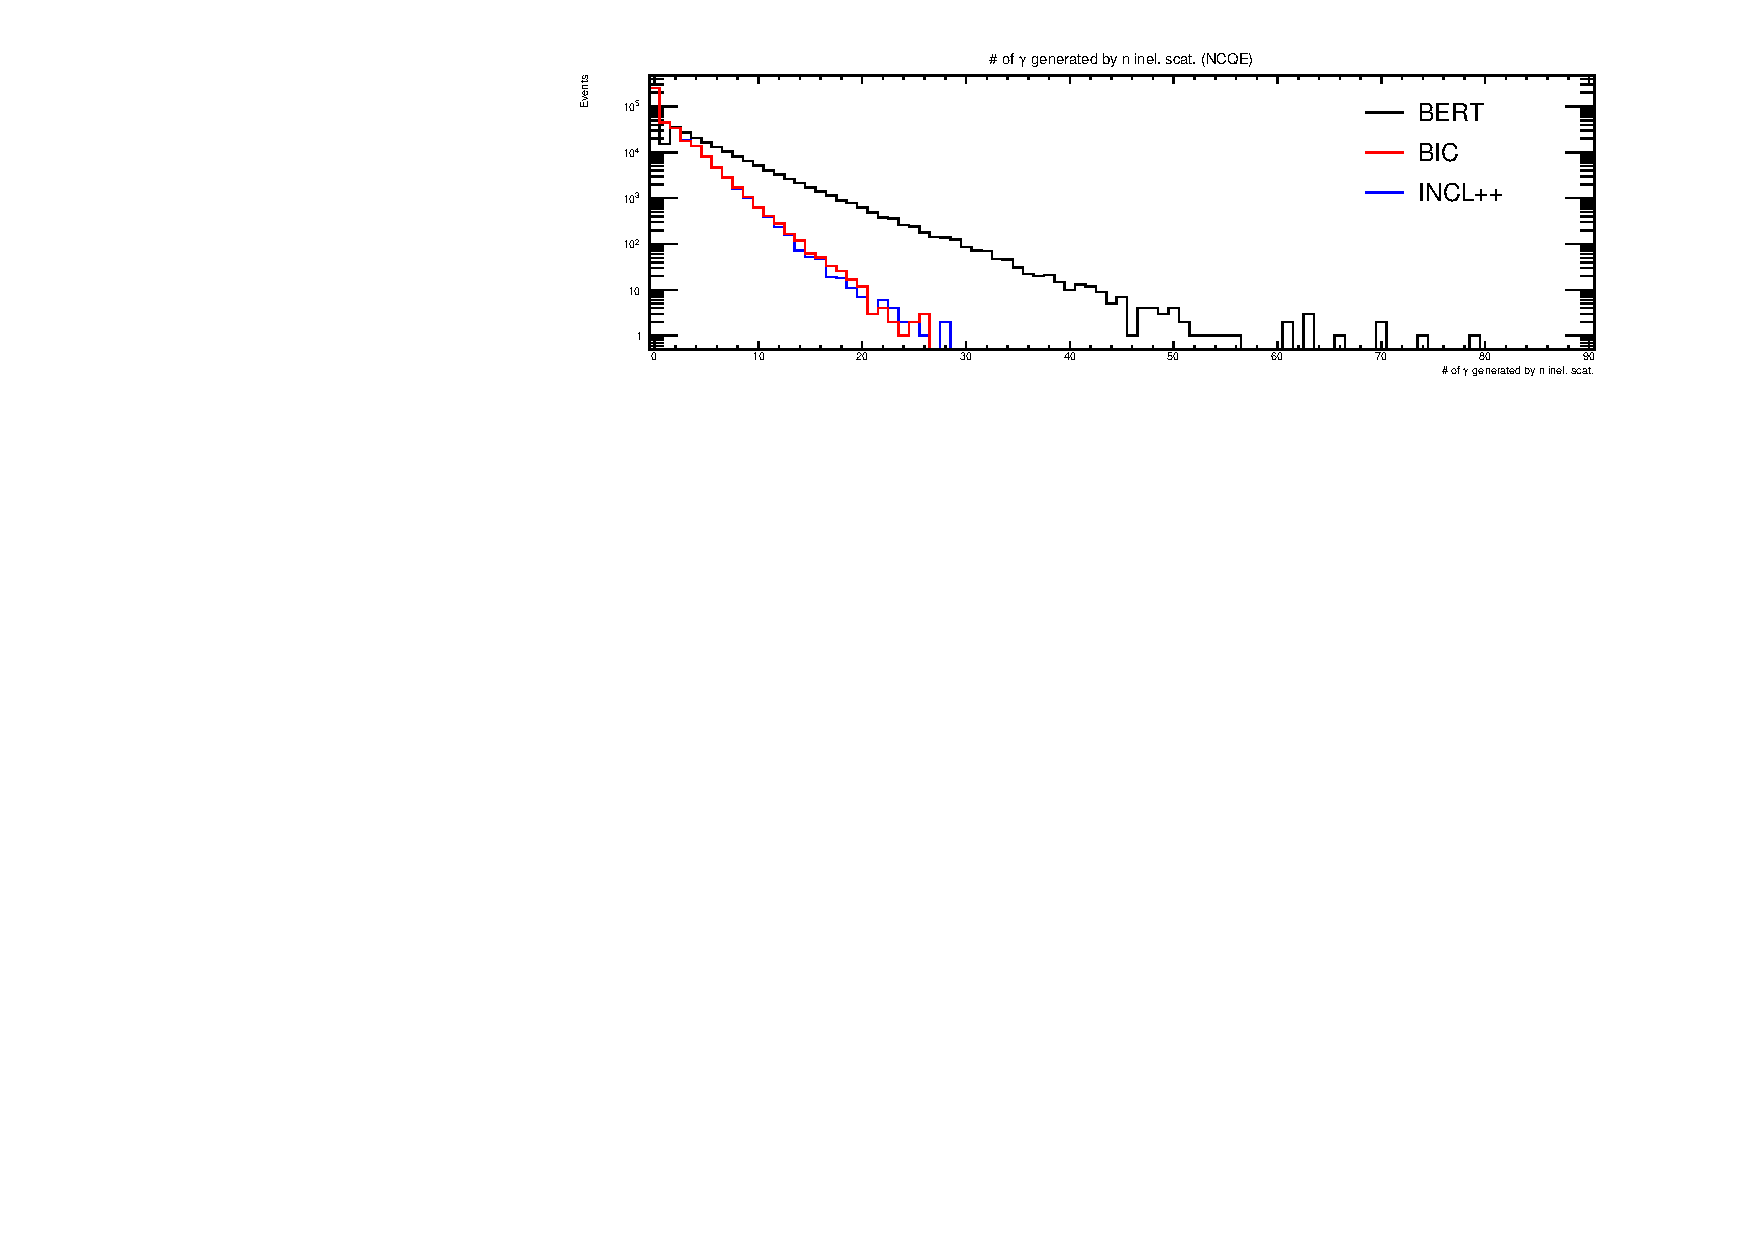
\includegraphics[width=16cm]{PDF/Secondary/Comparison/onlyNCQE_gamma/pdf1/Logy_NumSec}
	\caption[The number of gamma-rays generated by neutron inelastic scattering reactions]{
	The number of gamma-rays generated by neutron inelastic scattering reactions.
	Black, red, and blue line shows the case of BERT, BIC, and INCL++, respectively.
	}\label{gamma_Logy_NumSec}
\end{figure}

\begin{figure}[p]
	\centering
	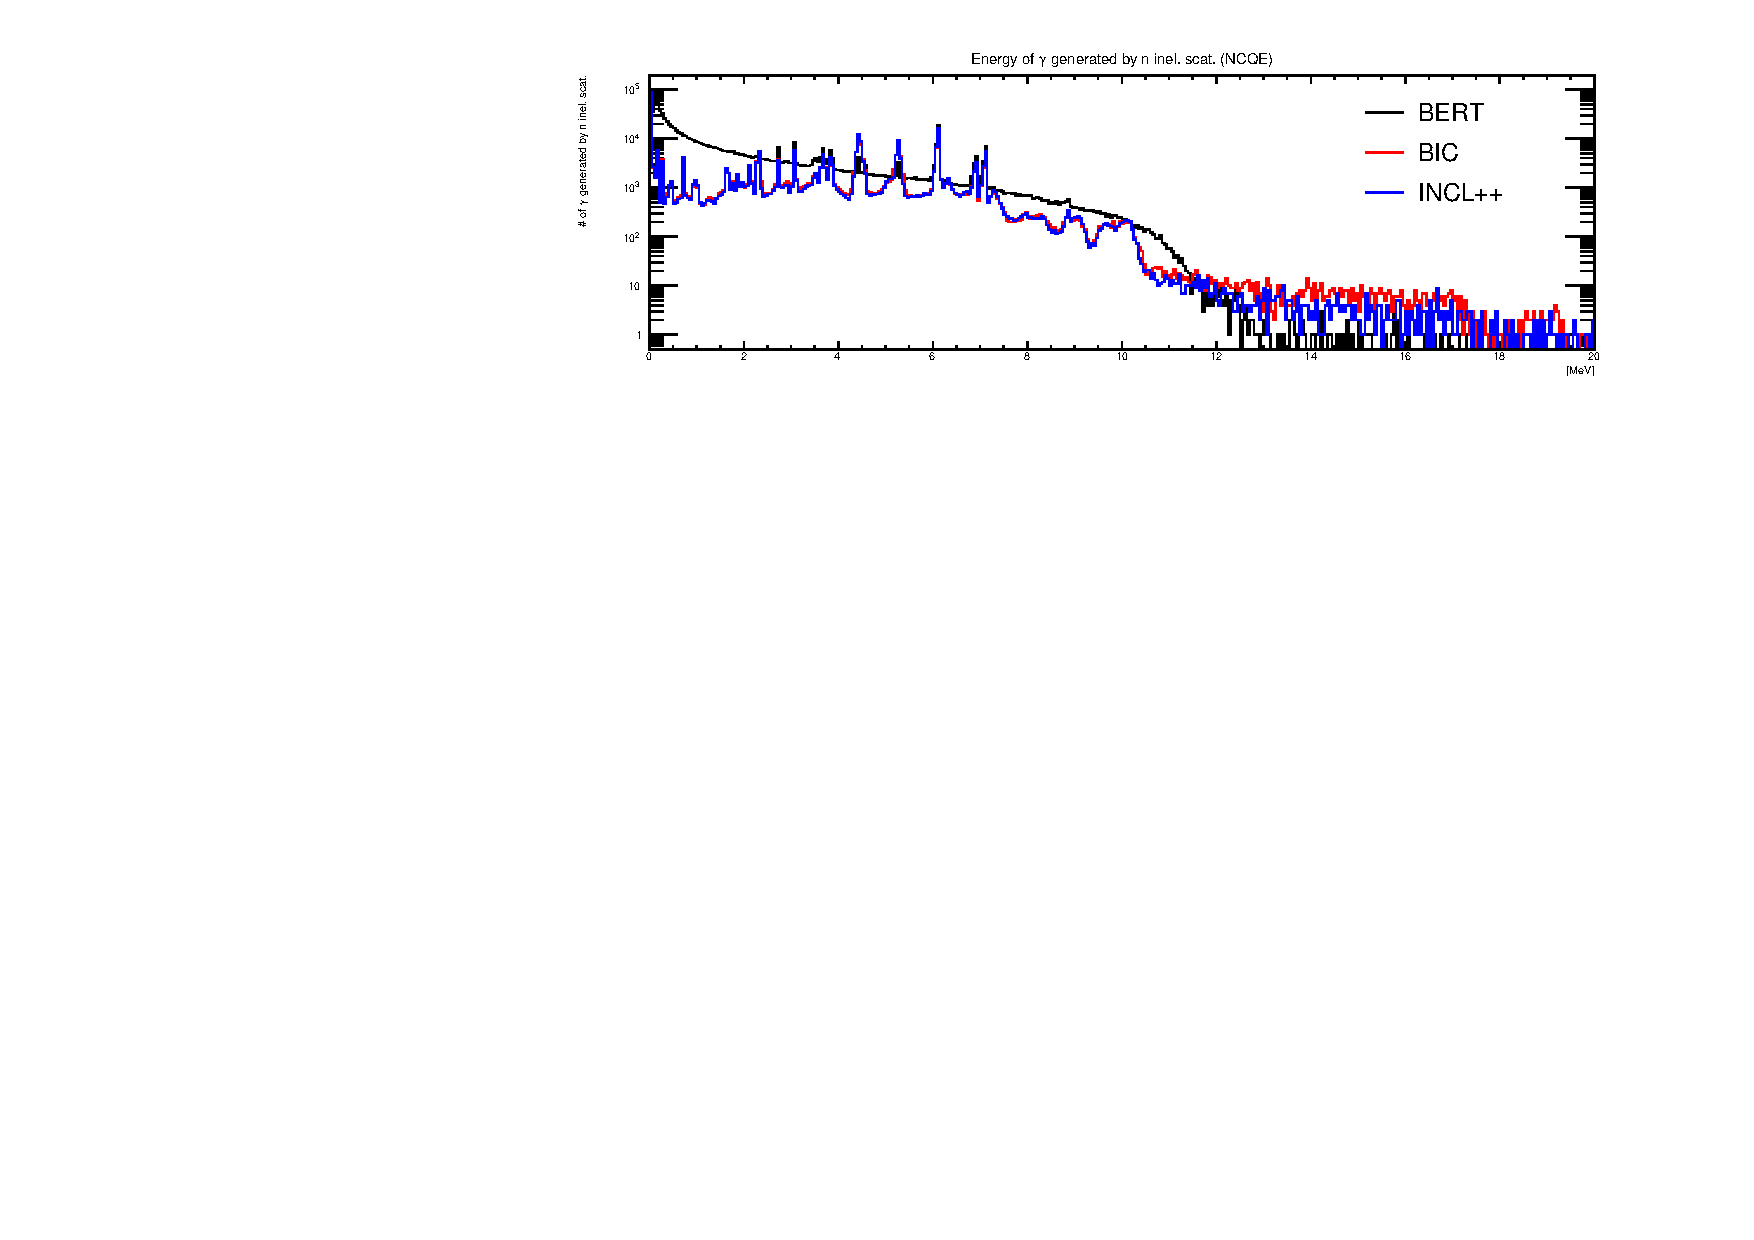
\includegraphics[width=16cm]{PDF/Secondary/Comparison/onlyNCQE_gamma/pdf1/Logy_EneSec}
	\caption[Energy of gamma-rays generated by neutron inelastic scattering reactions]{
	Energy of gamma-rays generated by neutron inelastic scattering reactions.
	Black, red, and blue line shows the case of BERT, BIC, and INCL++, respectively.
	}\label{gamma_Logy_EneSec}
\end{figure}

\begin{figure}[p]
	\centering
	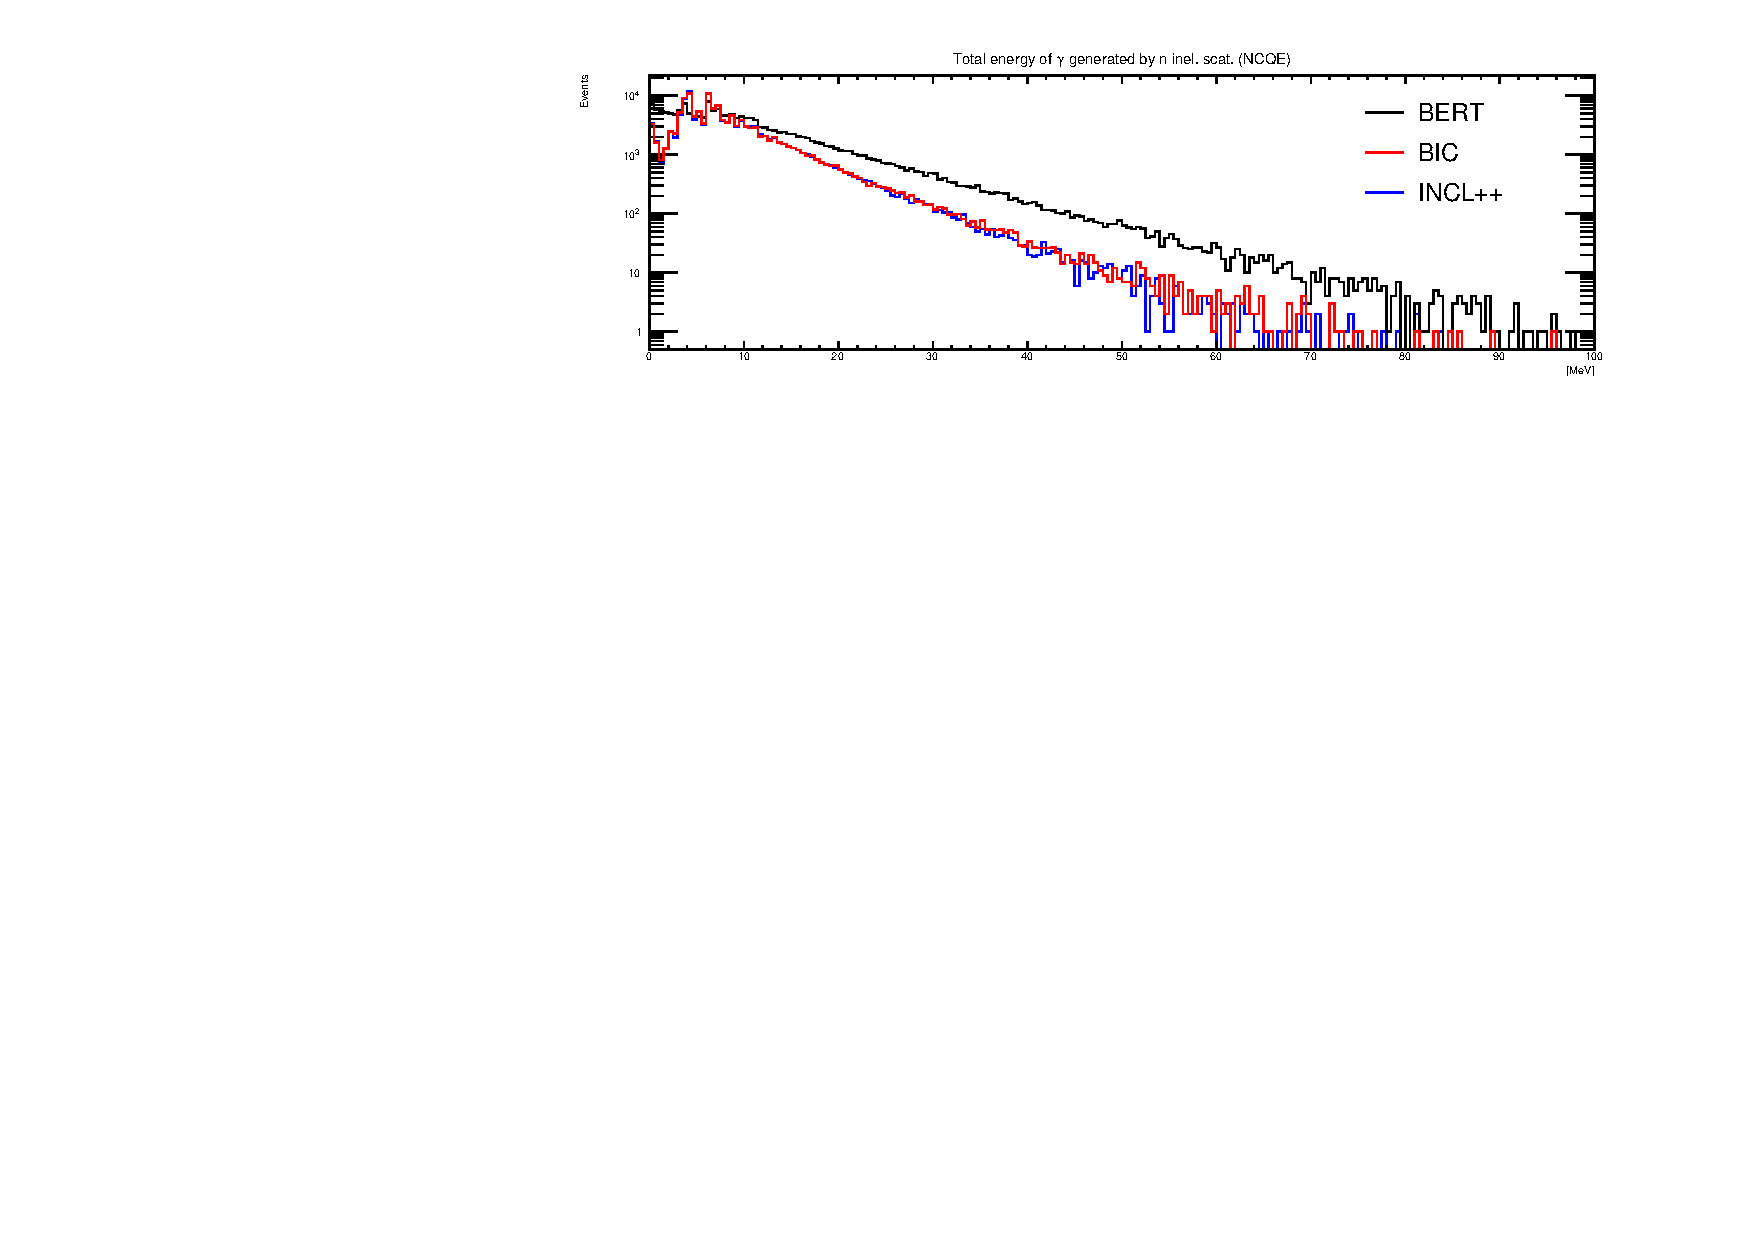
\includegraphics[width=16cm]{PDF/Secondary/Comparison/onlyNCQE_gamma/pdf1/Logy_TotEneSec}
	\caption[Total energy of gamma-rays generated by neutron inelastic scattering reactions]{
	Total energy of gamma-rays generated by neutron inelastic scattering reactions.
	Black, red, and blue line shows the case of BERT, BIC, and INCL++, respectively.
	}\label{gamma_Logy_TotEneSec}
\end{figure}

%\begin{table}[H]
%	\centering
%	\caption[The number of gamma-rays]{
%	The number of gamma-rays.
%	The number of primary gamma-rays is common among secondary interaction models.
%	}\label{tab:gamma}
%	\vs
%	\begin{tabular}{lrrr} \hline \hline
%		NCQE (383,284~events)                               &    BERT &     BIC &  INCL++ \\ \hline
%		The number of primary gamma-rays                    & 168,060 & 168,060 & 168,060 \\
%		The number of n inel. scat.                         & 458,254 & 409,019 & 396,804 \\
%		The number of gamma-rays per n inel. scat.          &  2.1599 &  0.8677 &  0.8902 \\
%		The number of gamma-rays by n inel. scat.           & 989,782 & 354,886 & 353,237 \\ \hline
%		The number of primary gamma-rays per event          &  0.4385 &  0.4385 &  0.4385 \\
%		The number of n inel. scat. per event               &  1.1956 &  1.0671 &  1.0353 \\
%		The number of gamma-rays by n inel. scat. per event &  2.5824 &  0.9259 &  0.9216 \\ \hline \hline
%	\end{tabular}
%\end{table}

\clearpage





\subsection{Differences of secondary interaction models}
\vs\hs
Secondary interactions can be described by the intranuclear-cascade model embedding the pre-compound (pre-equilibrium) model and evaporation (equilibrium) model.
Here, main differences of each model are described.
Details of each secondary interaction model are summarized in references cited below.

\subsubsection{Intranuclear-cascade model}
\vs
\textbf{Model category}\\
\hs
Intranuclear-cascade models can be categorized into two types.
One is a space-dependent intranuclear-cascade model, another is a time-dependent intranuclear-cascade model.
BERT belongs to the space-dependent intranuclear-cascade model, while BIC and INCL++ belong to the time-dependent intranuclear-cascade model.\\
\hs
In space-dependent intranuclear-cascade models, a collision point between a projectile and a target nucleon is determined by using the total particle-particle cross sections and region-dependent nucleon densities~\cite{Geant4}.
According to Ref.~\cite{2017KobraPhD}, the collision point $x$ is given by
\begin{eqnarray}
	x &=& -\lambda{\rm ln}\xi \nonumber \\
	  &=& -{1 \over \rho\sigma_{NN}}{\rm ln}\xi \nonumber \\
	  &=& -{A \over \rho\{Z\sigma_{N{\rm p}} + (A - Z)\sigma_{N{\rm n}}\}}{\rm ln}\xi,
\end{eqnarray}
where $\lambda$ is the mean free path, $\xi$ is the uniform random number between 0 and 1, $\rho$ is the nucleon density, $\sigma_{NN}$ is the nucleon-nucleon collision cross section, $A$ is the mass number (the number of nucleons), $Z$ is the atomic number (the number of protons), $\sigma_{N{\rm p}}$ is the collision cross section between the incoming particle and target proton, and $\sigma_{N{\rm n}}$ is the collision cross section between the incoming particle and target neutron.\\
\hs
In time-dependent intranuclear-cascade models, a distance of closest approach $d_{i}$ to each target nucleon $i$ is calculated using a straight line trajectory to determine a collision point~\cite{Geant4}.
According to Ref.~\cite{Geant4}, collisions will occur when $d_{i}$ satisfies the following inequality,
\begin{eqnarray}
	d_{i} < \sqrt{{\sigma_{i} \over \pi}},
\end{eqnarray}
where $\sigma_{i}$ is the total cross section.\\
\\
\textbf{Nuclear model}\\
\hs
Here, an oxygen nucleus ($A$ (mass number) $= 16$) is taken as an example.
In BERT, a nuclear model with three concentric spheres $i = \{1,2,3\}$ is used.
According to Ref.~\cite{Geant4}, the sphere radius is defined as
\begin{eqnarray}
	r_{i}(\alpha_{i}) = C_{2}\log\Bigg({1 + e^{-{C_{1} \over C_{2}}} \over \alpha_{i}} - 1\Bigg) + C_{1}\,\,\,(A > 11),
\end{eqnarray}
where $C_{1} = 3.3836A^{1/3}$, $C_{2} = 1.7234$, and $\alpha_{i} = \{0.01,0.3,0.7\}$.
Figure~\ref{Bertini_density} shows the nucleon-density distributions of $^{65}{\rm Cu}$~\cite{1963Bertini}.
The proton density in each region is set equal to the average value of the charge distribution in the region, and the neutron-to-proton density ratio in each region is equal to the neutron-to-proton ratio in the nucleus.

\begin{figure}[tbp]
	\centering
	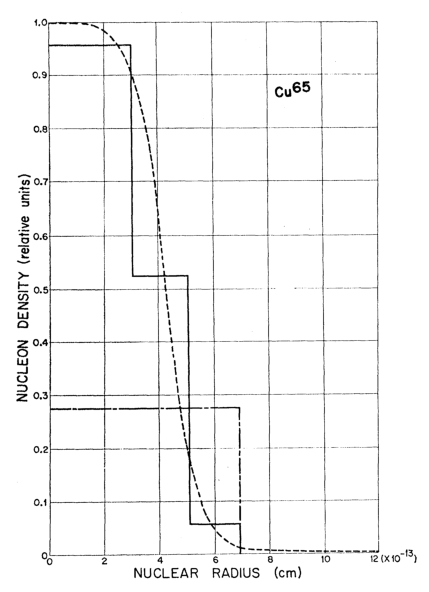
\includegraphics[width=6cm]{Figures/Model/Bertini_density}
	\caption[Nucleon-density distributions of $^{65}{\rm Cu}$]{
	Nucleon-density distributions of $^{65}{\rm Cu}$~\cite{1963Bertini}.
	Solid line, long-dash--short-dash line, and dashed line shows the standard three-region configulation, the uniform distribution, and Hofstadter's curve~\cite{1956Hofstadter}, respectively.
	}\label{Bertini_density}
\end{figure}

\hs
In BIC~\cite{Geant4}, the nucleon radii $r_{i}$ ($i = \{1,2,...,A\}$) are selected randomly according to the nucleon density $\rho(r_{i})$, and the nucleon density is given by
\begin{eqnarray}
	\rho(r_{i}) = (\pi R^{2})^{-3/2}\exp(-r_{i}^{2}/R^{2})\,\,\,(A < 17),
\end{eqnarray}
where $R^{2}=0.8133A^{2/3}\,{\rm fm}^{2}$.\\
\hs
In INCL++~\cite{2002Boudard}, the nucleon density is given by
\begin{eqnarray}
	\rho(r) = \left\{
	\begin{array}{ll}
		{\rho_{0} \over 1\,+\,\exp\big({r - R_{0} \over a}\big)} & ({\rm for}\,r < R_{\rm max}) \\
		0                                                        & ({\rm for}\,r > R_{\rm max})
	\end{array} \right. ,
\end{eqnarray}
where $R_{0} = (2.745 \times 10^{-4}A + 1.063)A^{1/3}\,{\rm fm}$, $a = 0.510 + 1.63 \times 10^{-4}A\,{\rm fm}$, and $R_{\rm max} = R_{0} + 8a$.
The quantity $\rho_{0}$ is like that the distribution is normalized to $A$.\\
\\
\textbf{Stopping time}\\
\hs
In BERT and BIC~\cite{Geant4}, the cascade ends when all particles which can escape the nucleus, have done so.\\
\hs
While, in INCL++~\cite{Geant4}, the cascade stopping time $t_{\rm stop}$ is defined as
\begin{eqnarray}
	t_{\rm stop} = t_{0}\bigg({A \over 208}\bigg)^{0.16},
\end{eqnarray}
where $t_{0}=70~{\rm fm}/c$.
The cascade also ends if no participants are left in the nucleus.
Figure~\ref{INCL_time} shows the time variation of four physical quantities obtained by collisions of 1-GeV protons with Pb nuclei in INCL++~\cite{2002Boudard}.
In this figure, arrows show the stopping time, and the stopping time is about $70~{\rm fm}/c$ because the target nucleus is Pb ($A \sim 208$).

\begin{figure}[H]
	\centering
	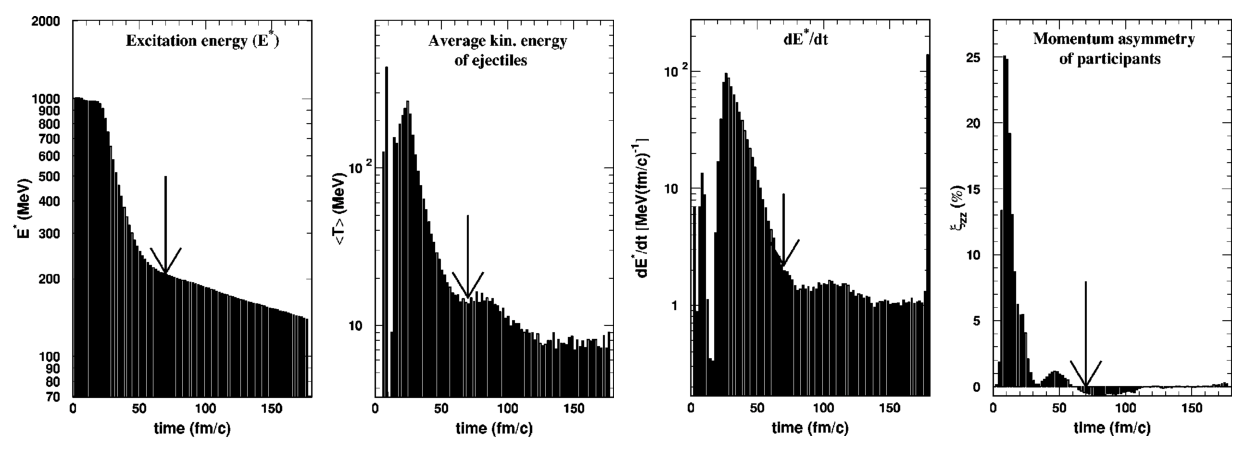
\includegraphics[width=16cm]{Figures/Model/INCL_time}
	\caption[Time variation of four physical quantities obtained by collisions of 1-GeV protons with Pb nuclei in INCL++]{
	Time variation of four physical quantities obtained by collisions of 1-GeV protons with Pb nuclei in INCL++~\cite{2002Boudard}.
	Left, center left, center right, and right figure shows the time variation of excitation energy, average kinetic energy of ejectiles, time derivative of the excitation energy, and momentum asymmetry of participants, respectively.
	The arrows show the stopping time.
	}\label{INCL_time}
\end{figure}

\subsubsection{Pre-compound model and evaporation model}
\vs\hs
BERT embeds its own pre-compound and evaporation models, while BIC and INCL++ embed Geant4 native pre-compound and evaporation models~\cite{2011Quesada}.
However, as a option, BERT can switch to the Geant4 native pre-compound and evaporation models.
Therefore, we confirmed some distributions shown in Section~\ref{Subsec_Features} using BERT embedding the Geant4 native pre-compound and evaporation models.
Figure~\ref{Pre_gamma_NumSecIne} shows the number of generated gamma-rays per neutron inelastic scattering reaction.
From this figure, we can confirm that the shape of the distribution in BERT with the Geant4 pre-compound model is much closer to that in BIC and INCL++ compared to Figure~\ref{gamma_NumSecIne}.
The number of gamma-rays generated by neutron inelastic scattering reactions is also close between BERT with the Geant4 pre-compound model and BIC and INCL++, as shown in Figure~\ref{Pre_gamma_Logy_NumSec}.
Furthermore, as shown in Figure~\ref{Pre_gamma_Logy_EneSec} and Figure~\ref{Pre_gamma_Logy_TotEneSec}, energy and total energy of gamma-rays generated by neutron inelastic scattering reactions are also close among these models.
The numbers of neutrons, neutron captures, and gamma-rays are summarized in Table~\ref{tab:pre_gamma}.\\
\hs
The main difference between models embedded in BERT and Geant4 native models seems to be the condition under which the evaporation process ends.
According to Ref.~\cite{Geant4}, in evaporation model embedded in BERT, the main chain of evaporation is followed until an excitation energy falls below $E_{\rm cutoff} = 0.1\,{\rm MeV}$, and a gamma-ray emission chain continues until the excitation energy is less than $E^{\gamma}_{\rm cutoff} = 10^{-15}\,{\rm MeV}$.
By this specification, the numbers of neutrons and gamma-rays are considered to be larger in BERT that embeds its own pre-compound and evaporation models.

\begin{figure}[h]
	\centering
	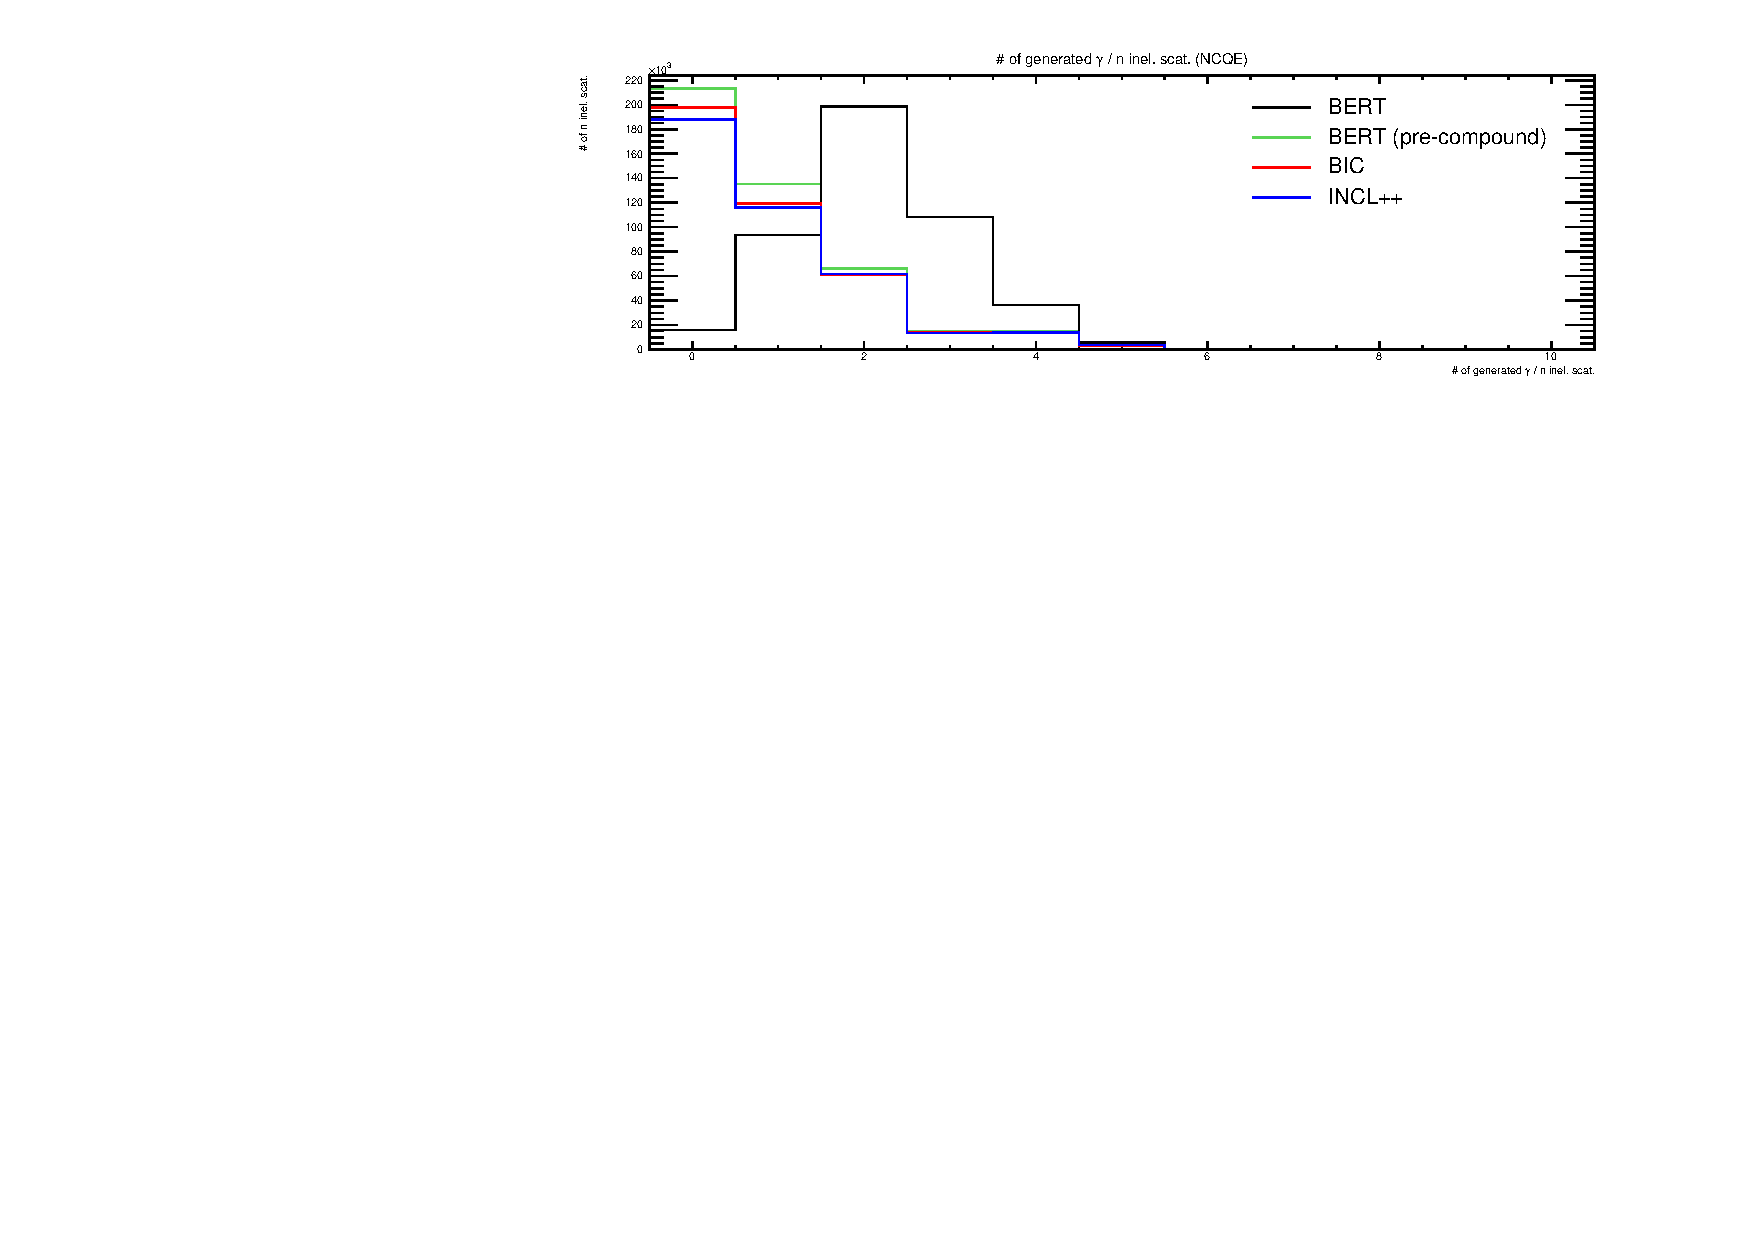
\includegraphics[width=16cm]{PDF/Secondary/Comparison_PreCompound/onlyNCQE_gamma/pdf1/NumSecIne}
	\caption[The number of generated gamma-rays per neutron inelastic scattering reaction]{
	The number of generated gamma-rays per neutron inelastic scattering reaction.
	Black, green, red, and blue line shows the case of BERT, BERT with the Geant4 pre-compound model, BIC, and INCL++, respectively.
	}\label{Pre_gamma_NumSecIne}
\end{figure}

\begin{figure}[h]
	\centering
	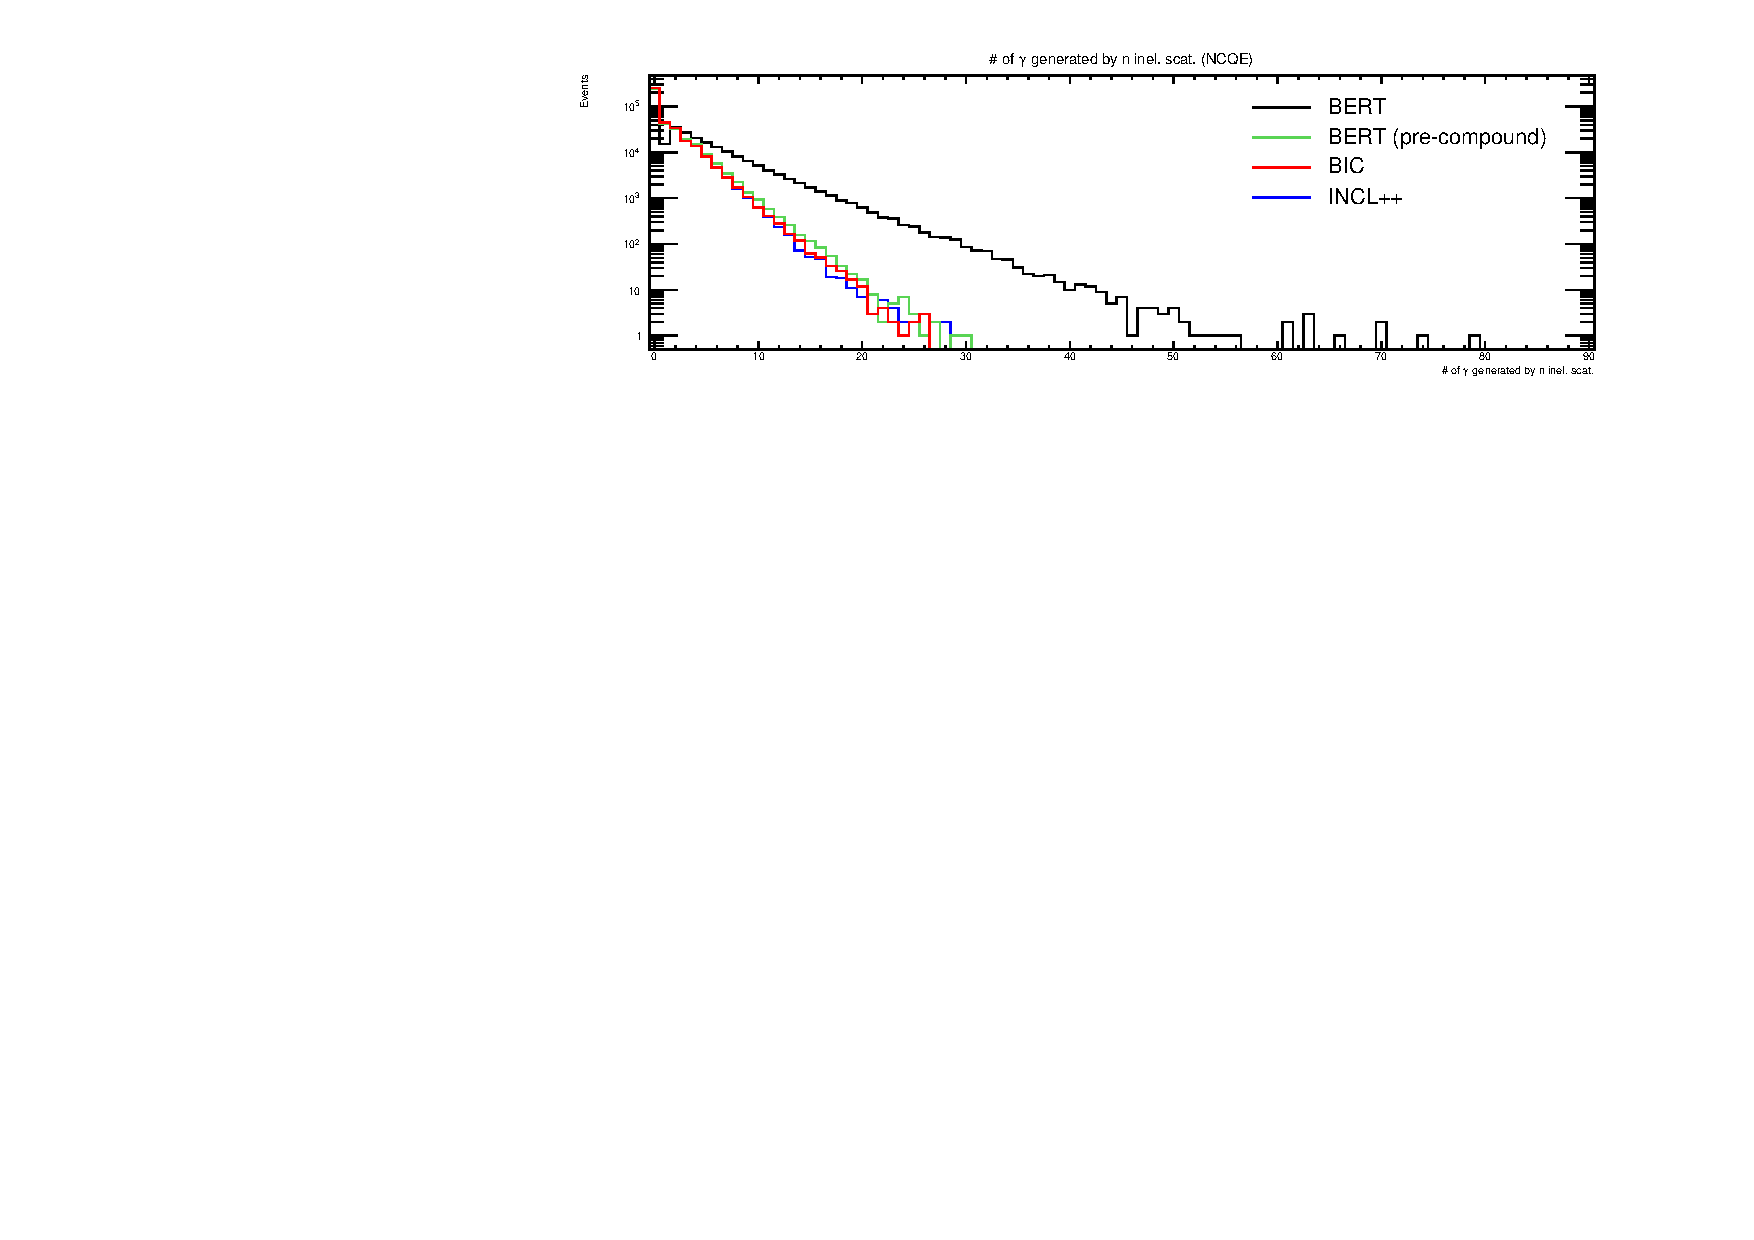
\includegraphics[width=16cm]{PDF/Secondary/Comparison_PreCompound/onlyNCQE_gamma/pdf1/Logy_NumSec}
	\caption[The number of gamma-rays generated by neutron inelastic scattering reactions]{
	The number of gamma-rays generated by neutron inelastic scattering reactions.
	Black, green, red, and blue line shows the case of BERT, BERT with the Geant4 pre-compound model, BIC, and INCL++, respectively.
	}\label{Pre_gamma_Logy_NumSec}
\end{figure}

\begin{figure}[h]
	\centering
	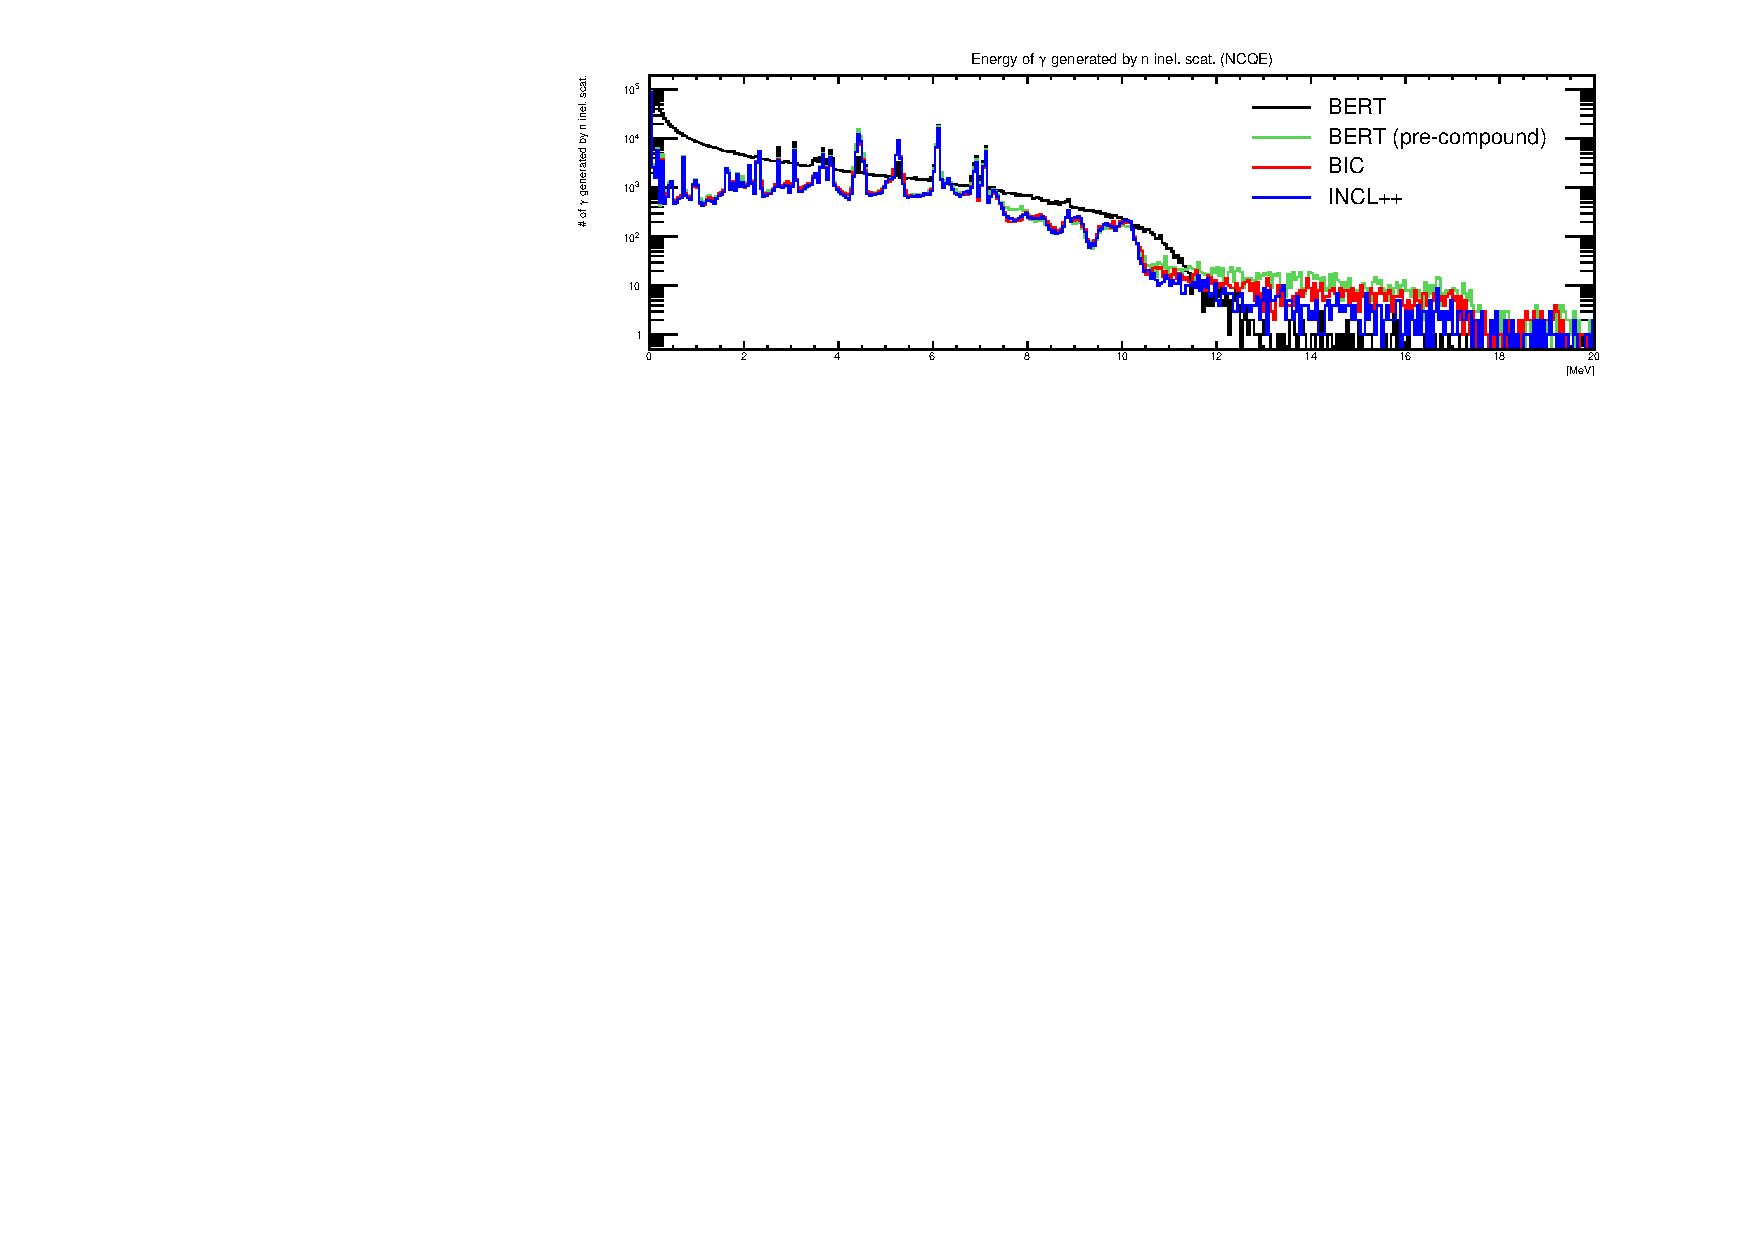
\includegraphics[width=16cm]{PDF/Secondary/Comparison_PreCompound/onlyNCQE_gamma/pdf1/Logy_EneSec}
	\caption[Energy of gamma-rays generated by neutron inelastic scattering reactions]{
	Energy of gamma-rays generated by neutron inelastic scattering reactions.
	Black, green, red, and blue line shows the case of BERT, BERT with the Geant4 pre-compound model, BIC, and INCL++, respectively.
	}\label{Pre_gamma_Logy_EneSec}
\end{figure}

\begin{figure}[h]
	\centering
	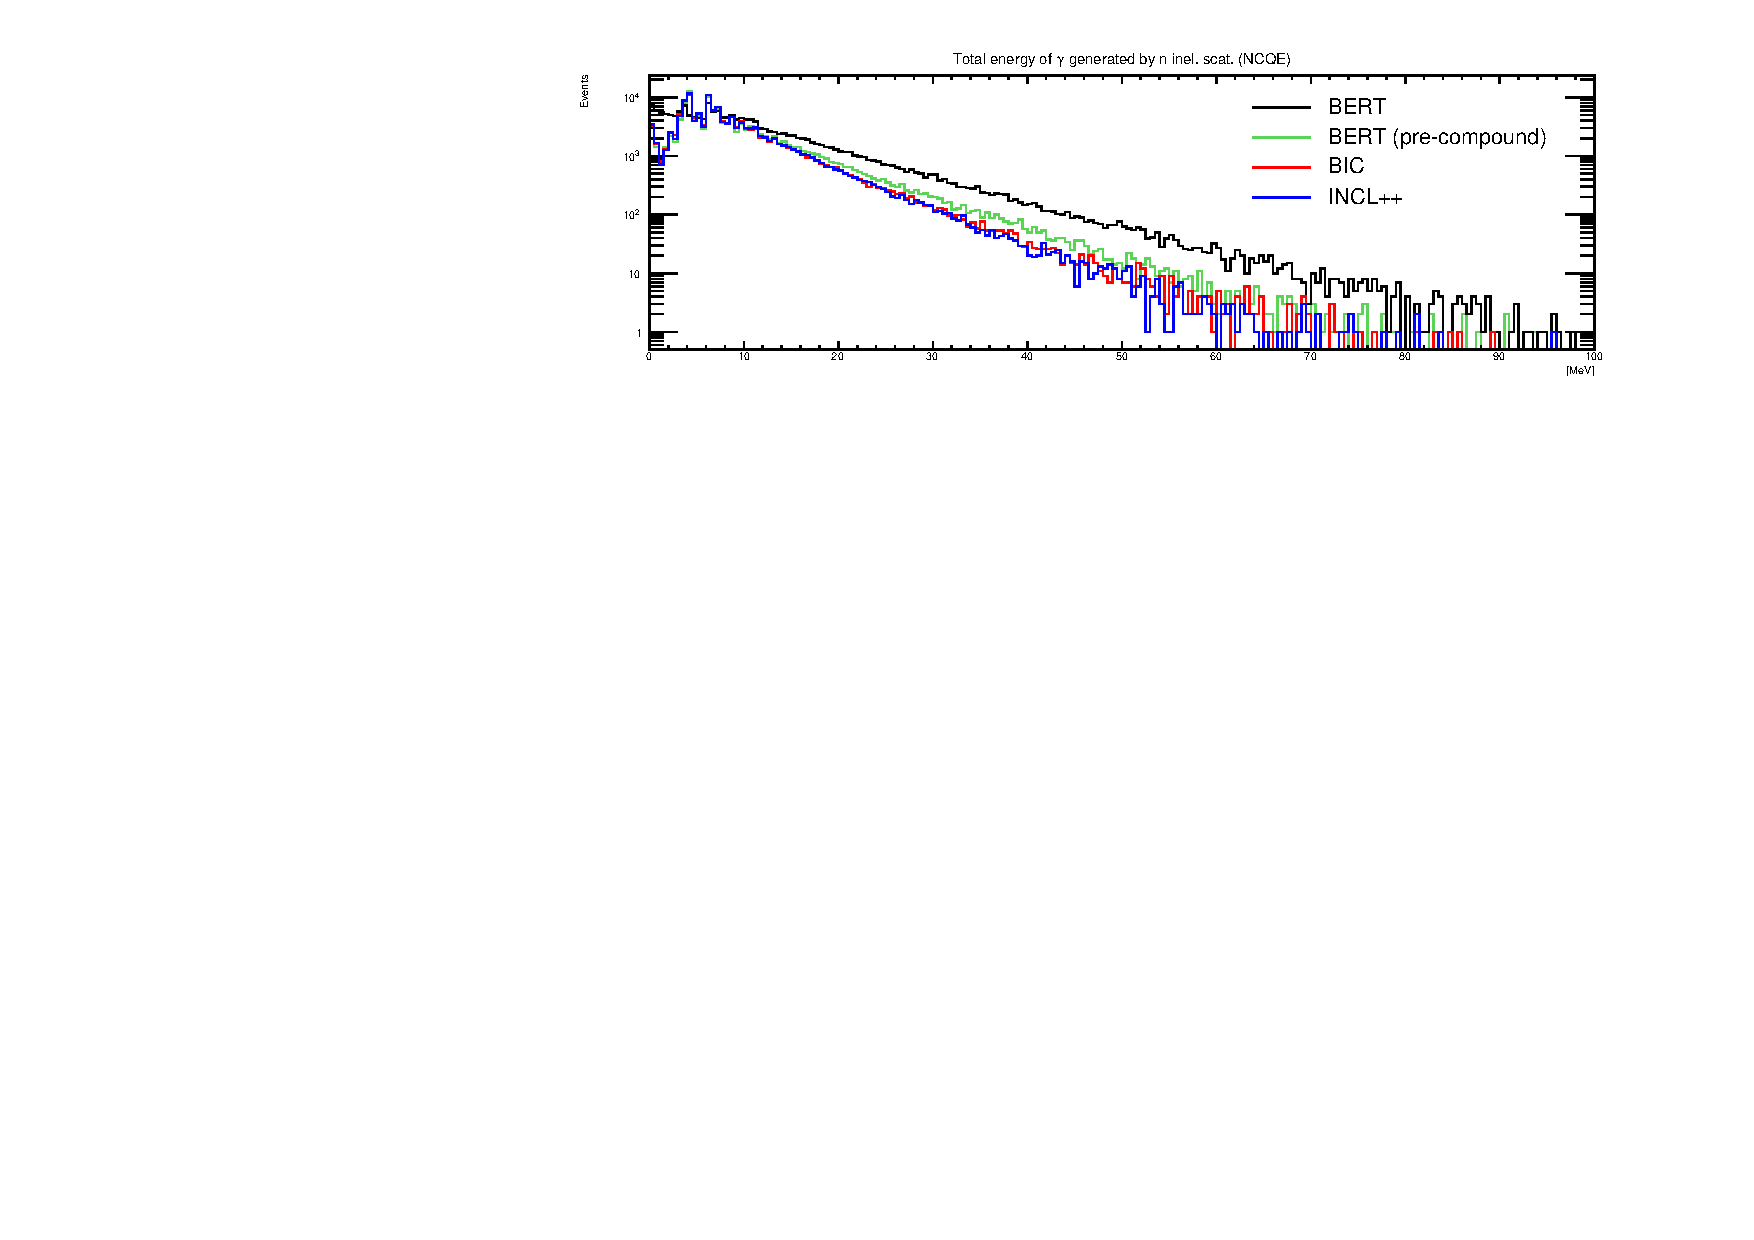
\includegraphics[width=16cm]{PDF/Secondary/Comparison_PreCompound/onlyNCQE_gamma/pdf1/Logy_TotEneSec}
	\caption[Total energy of gamma-rays generated by neutron inelastic scattering reactions]{
	Total energy of gamma-rays generated by neutron inelastic scattering reactions.
	Black, green, red, and blue line shows the case of BERT, BERT with the Geant4 pre-compound model, BIC, and INCL++, respectively.
	}\label{Pre_gamma_Logy_TotEneSec}
\end{figure}

\begin{table}[h]
	\centering
	\caption[The number of neutrons generated by each process, the total number of neutrons and neutron captures, and the number of gamma-rays]{
	The number of neutrons generated by each process (top), the total number of neutrons and neutron captures (center), and the number of gamma-rays (bottom).
%	In each table, a column of BERT with the Geant4 pre-compound model is added.
	The numbers of primary neutrons and primary gamma-rays are common among secondary interaction models.
	}\label{tab:pre_gamma}
	\vs
	\begin{tabular}{lrrrr} \hline \hline
		NCQE (383,284~events)                               &    BERT &           BERT &     BIC &  INCL++ \\
		                                                    &         & (pre-compound) &         &         \\ \hline
		neutron inelastic scattering                        & 178,029 &        131,337 & 124,582 & 107,027 \\
		proton inelastic scattering                         &  36,295 &         29,613 &  39,112 &  34,040 \\
		$\pi^{+}$ inelastic scattering                      &     349 &            322 &     297 &     285 \\
		$\pi^{-}$ inelastic scattering                      &     638 &            592 &     785 &     722 \\
		$\mu^{-}$ capture                                   &      10 &              9 &      15 &      12 \\
		$\pi^{-}$ capture                                   &   4,221 &          4,155 &   4,548 &   4,693 \\
		gamma-nuclear interaction                           &      64 &             42 &      61 &      61 \\
		others                                              &     196 &            169 &      45 &   2,164 \\ \hline
		The number of generated neutrons                    & 219,802 &        166,239 & 169,445 & 149,004 \\ \hline
		The number of generated neutrons per event          &  0.5735 &         0.4337 &  0.4421 &  0.3888 \\ \hline \hline
		&&& \\ \hline \hline
		NCQE (383,284~events)                               &    BERT &           BERT &     BIC &  INCL++ \\
		                                                    &         & (pre-compound) &         &         \\ \hline
		The number of primary neutrons                      & 310,835 &        310,835 & 310,835 & 310,835 \\
		The number of generated neutrons                    & 219,802 &        166,239 & 169,445 & 149,004 \\
		The total number of neutrons                        & 530,637 &        477,074 & 480,280 & 459,839 \\
		The number of neutron captures                      & 495,346 &        425,718 & 411,087 & 405,483 \\ \hline
		The number of primary neutrons per event            &  0.8110 &         0.8110 &  0.8110 &  0.8110 \\
		The number of generated neutrons per event          &  0.5735 &         0.4337 &  0.4421 &  0.3888 \\
		The total number of neutrons per event              &  1.3844 &         1.2447 &  1.2531 &  1.1997 \\
		The number of neutron captures per event            &  1.2924 &         1.1107 &  1.0725 &  1.0579 \\ \hline \hline
		&&& \\ \hline \hline
		NCQE (383,284~events)                               &    BERT &           BERT &     BIC &  INCL++ \\
		                                                    &         & (pre-compound) &         &         \\ \hline
		The number of primary gamma-rays                    & 168,060 &        168,060 & 168,060 & 168,060 \\
		The number of n inel. scat.                         & 458,254 &        448,775 & 409,019 & 396,804 \\
		The number of gamma-rays per n inel. scat.          &  2.1599 &         0.8727 &  0.8677 &  0.8902 \\
		The number of gamma-rays by n inel. scat.           & 989,782 &        391,633 & 354,886 & 353,237 \\ \hline
		The number of primary gamma-rays per event          &  0.4385 &         0.4385 &  0.4385 &  0.4385 \\
		The number of n inel. scat. per event               &  1.1956 &         1.1709 &  1.0671 &  1.0353 \\
		The number of gamma-rays by n inel. scat. per event &  2.5824 &         1.0218 &  0.9259 &  0.9216 \\ \hline \hline
	\end{tabular}
\end{table}





\clearpage
\subsection{Comparison with the observed data}\label{Subsec_Comp_data}
\vs\hs
Figure~\ref{Comparison_Figure02_Poisson}, Figure~\ref{Comparison_Figure08_Poisson}, and Figure~\ref{Comparison_Figure04_Poisson} show the distributions of $\theta_{\rm C}$, $E_{\rm vis}$, and $N_{\rm delayed}$ in each secondary interaction model, respectively.
The distributions of $\theta_{\rm C}$, $E_{\rm vis}$, and $N_{\rm delayed}$ strongly depend on the number of de-excitation gamma-rays and neutrons.
For example, the direction of Cherenkov photons becomes more isotropic as the number of de-excitation gamma-rays is increased.
Moreover, the total energy of de-excitation gamma-rays is correlated to the number of de-excitation gamma-rays.
Therefore, $\theta_{\rm C}$ and $E_{\rm vis}$ become larger as the number of de-excitation gamma-rays gets larger.
Furthermore, $N_{\rm delayed}$ is correlated to the total number of neutrons.\\
\hs
In Figure~\ref{Comparison_Figure08_Poisson} ($E_{\rm vis}$ distribution) and Figure~\ref{Comparison_Figure04_Poisson} ($N_{\rm delayed}$ distribution), the number of events becomes larger in BERT than other two models.
Furthermore, in Figure~\ref{Comparison_Figure02_Poisson} ($\theta_{\rm C}$ distribution), the differences between BERT and other two models are large in high-angle regions.
These differences come from the number of de-excitation gamma-rays and neutrons by secondary interactions, which is described in Section~\ref{Subsec_Features}.
The number of de-excitation gamma-rays and neutrons is similar between BIC and INCL++.
While, in BERT, the number of de-excitation gamma-rays and neutrons is larger than in the other two models.

%\begin{figure}[b]
%	\centering
%	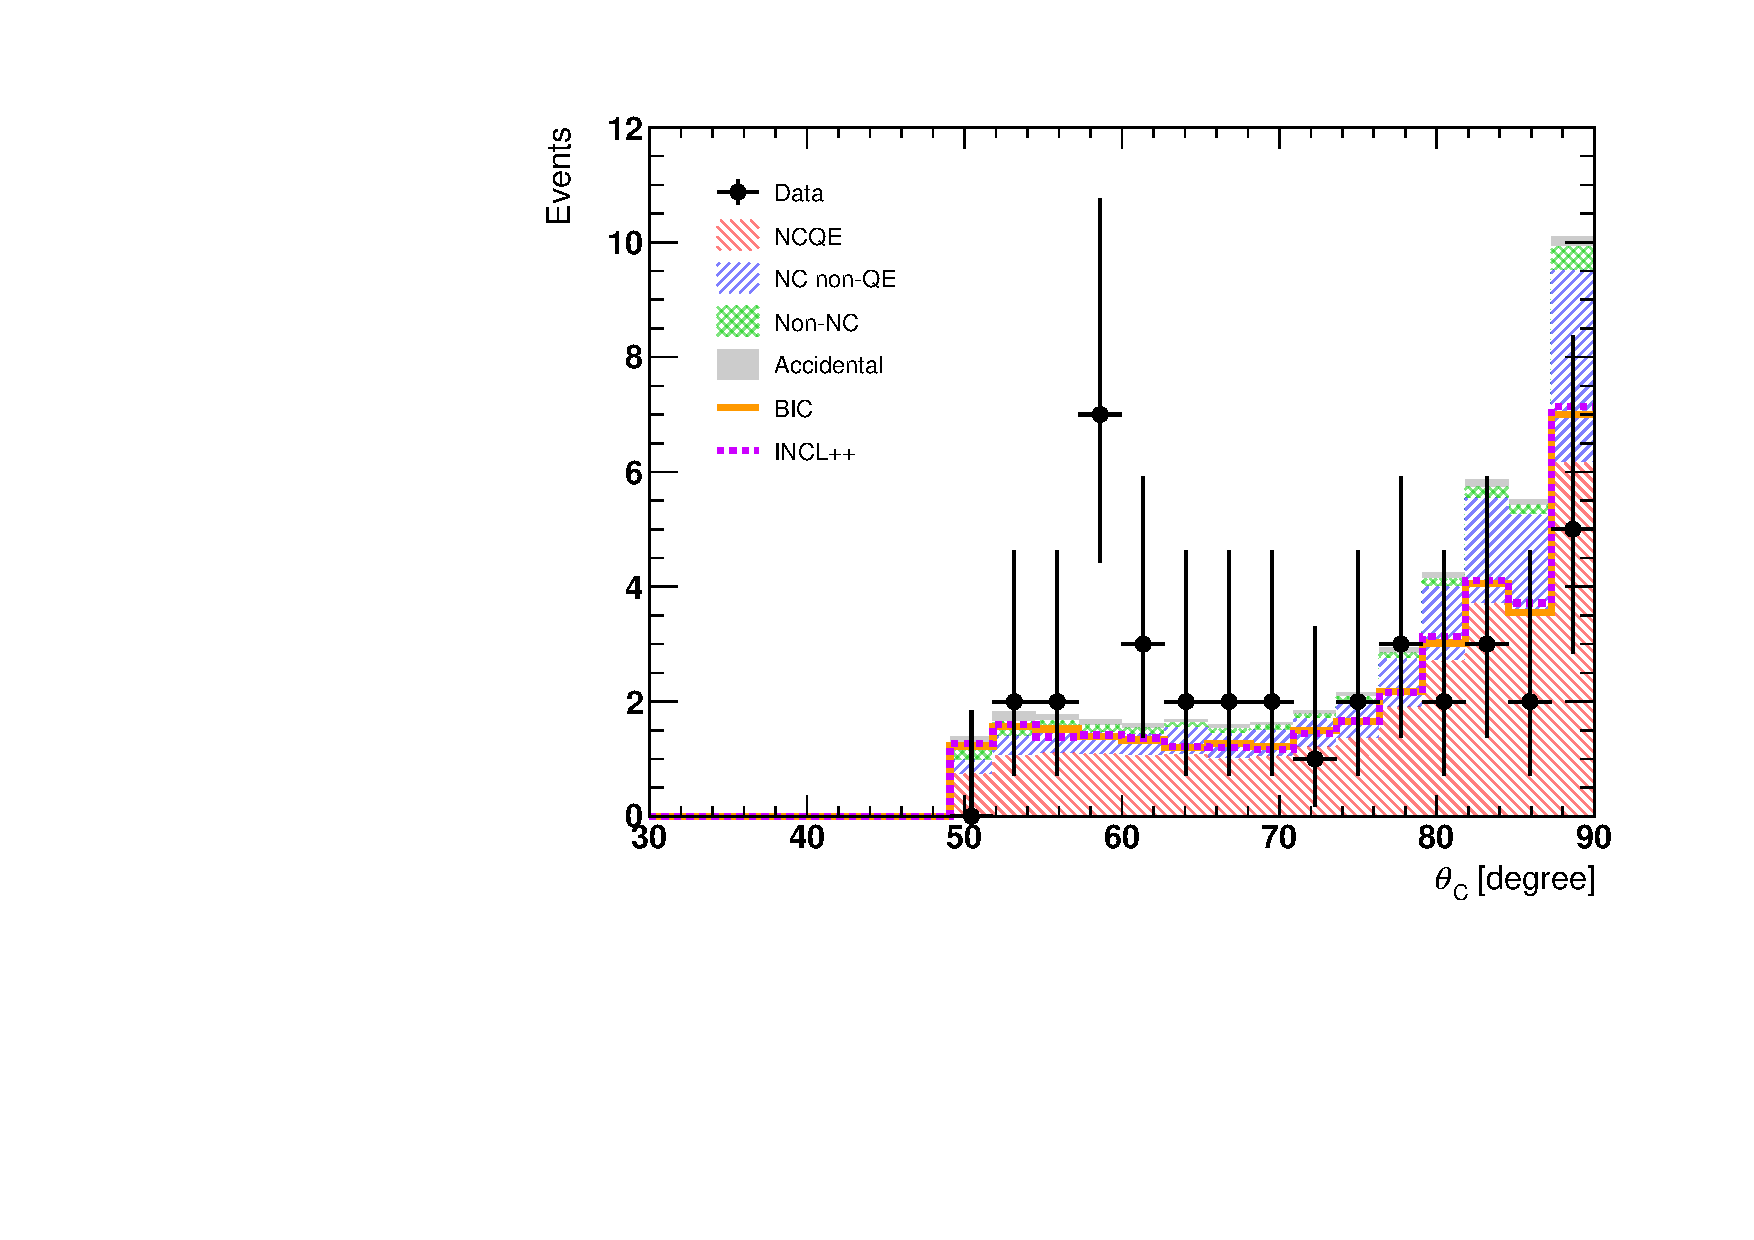
\includegraphics[width=12cm]{PDF/Figure02_02/Comparison/Figure02_Poisson}
%	\caption[$\theta_{\rm C}$ distribution]{
%	$\theta_{\rm C}$ distribution.
%	Each color-filled histogram shows the expected events in BERT.
%	Non-NC includes CC, spallation, and reactor neutrino events.
%	Solid and dashed line show the total expected events in BIC and INCL++, respectively.
%	In this distribution, $E_{\rm vis}$ is between 7.49~MeV and 29.49~MeV and $N_{\rm delayed}$ is greater or equal to one.
%	}\label{Comparison_Figure02_Poisson}
%\end{figure}

%\begin{figure}[b]
%	\centering
%	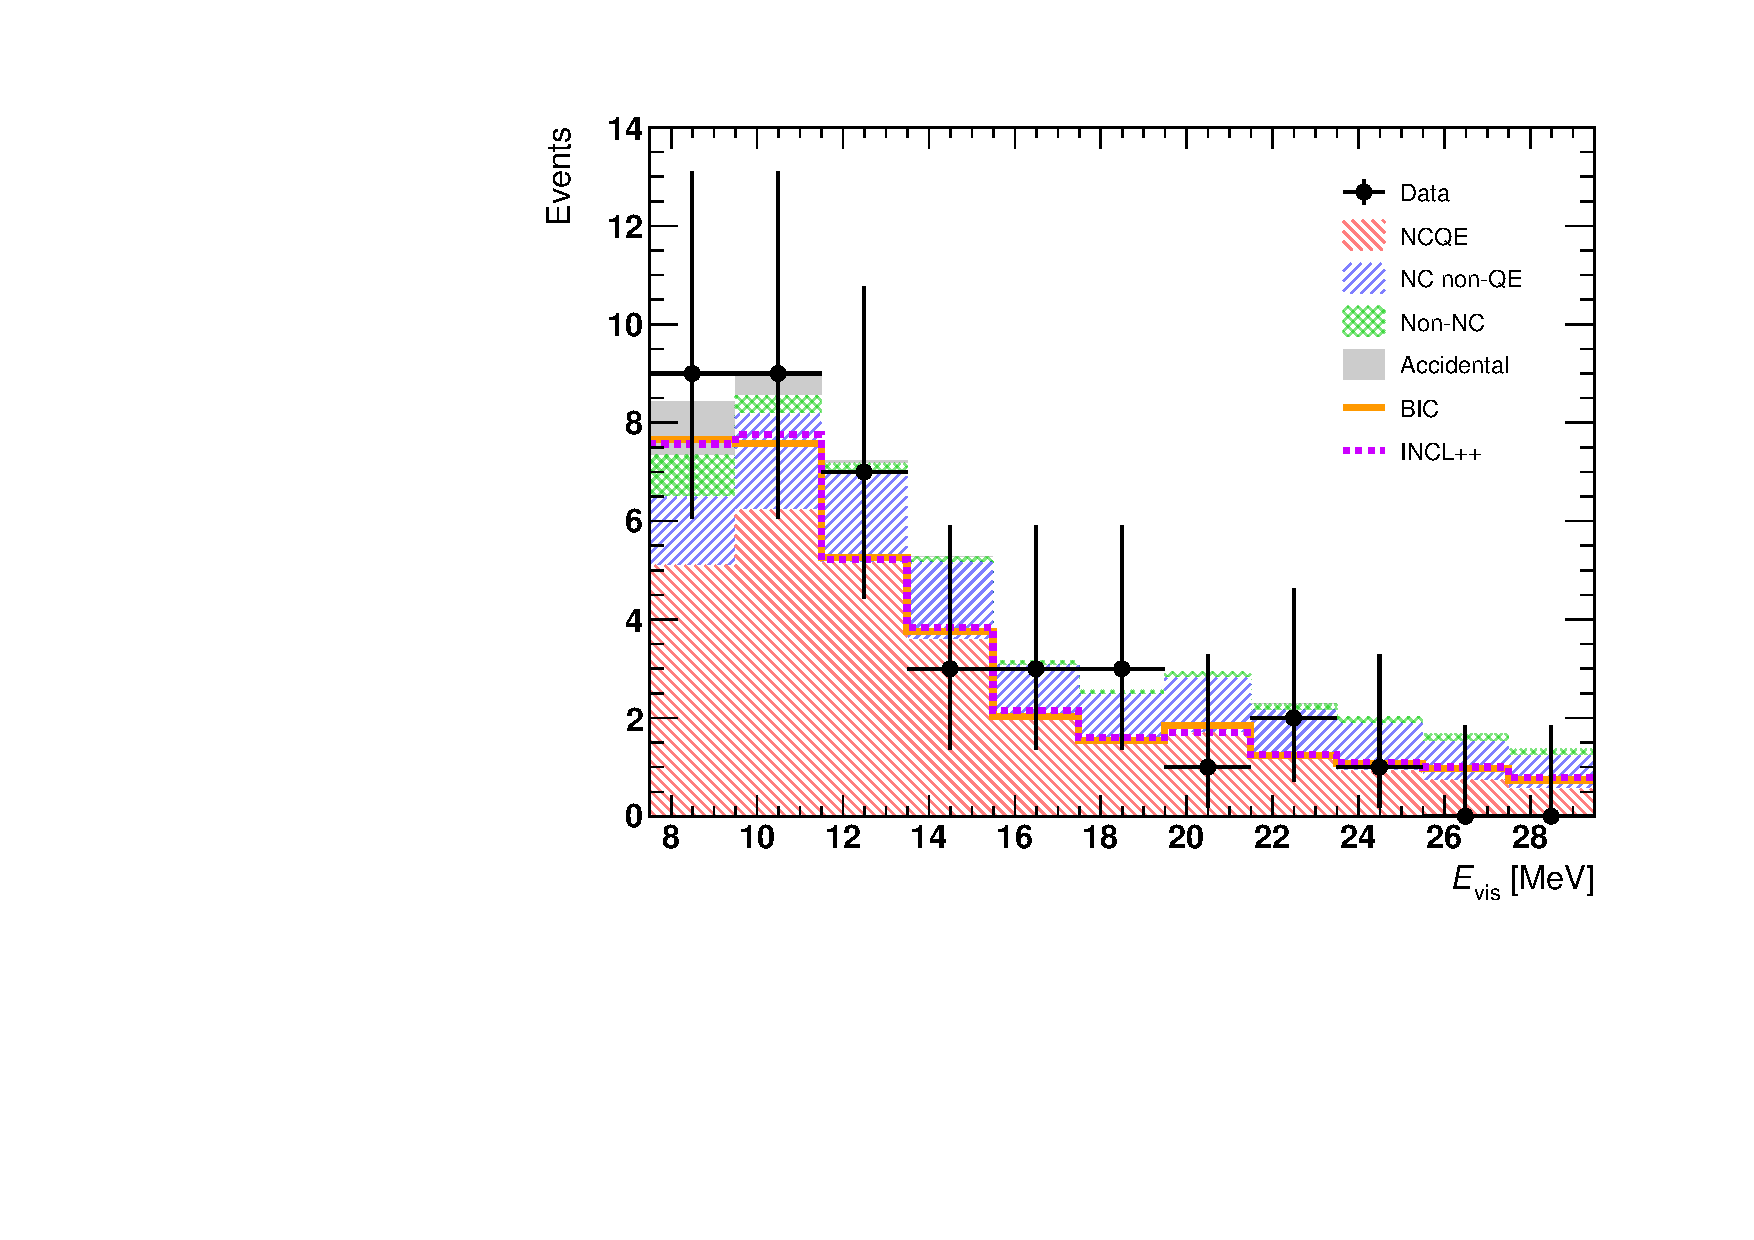
\includegraphics[width=12cm]{PDF/Figure08/Comparison/Figure08_Poisson}
%	\caption[$E_{\rm vis}$ distribution]{
%	$E_{\rm vis}$ distribution.
%	Each color-filled histogram shows the expected events in BERT.
%	Non-NC includes CC, spallation, and reactor neutrino events.
%	Solid and dashed line show the total expected events in BIC and INCL++, respectively.
%	In this distribution, $\theta_{\rm C}$ is greater than 50~degrees and $N_{\rm delayed}$ is greater or equal to one.
%	}\label{Comparison_Figure08_Poisson}
%\end{figure}

%\begin{figure}[b]
%	\centering
%	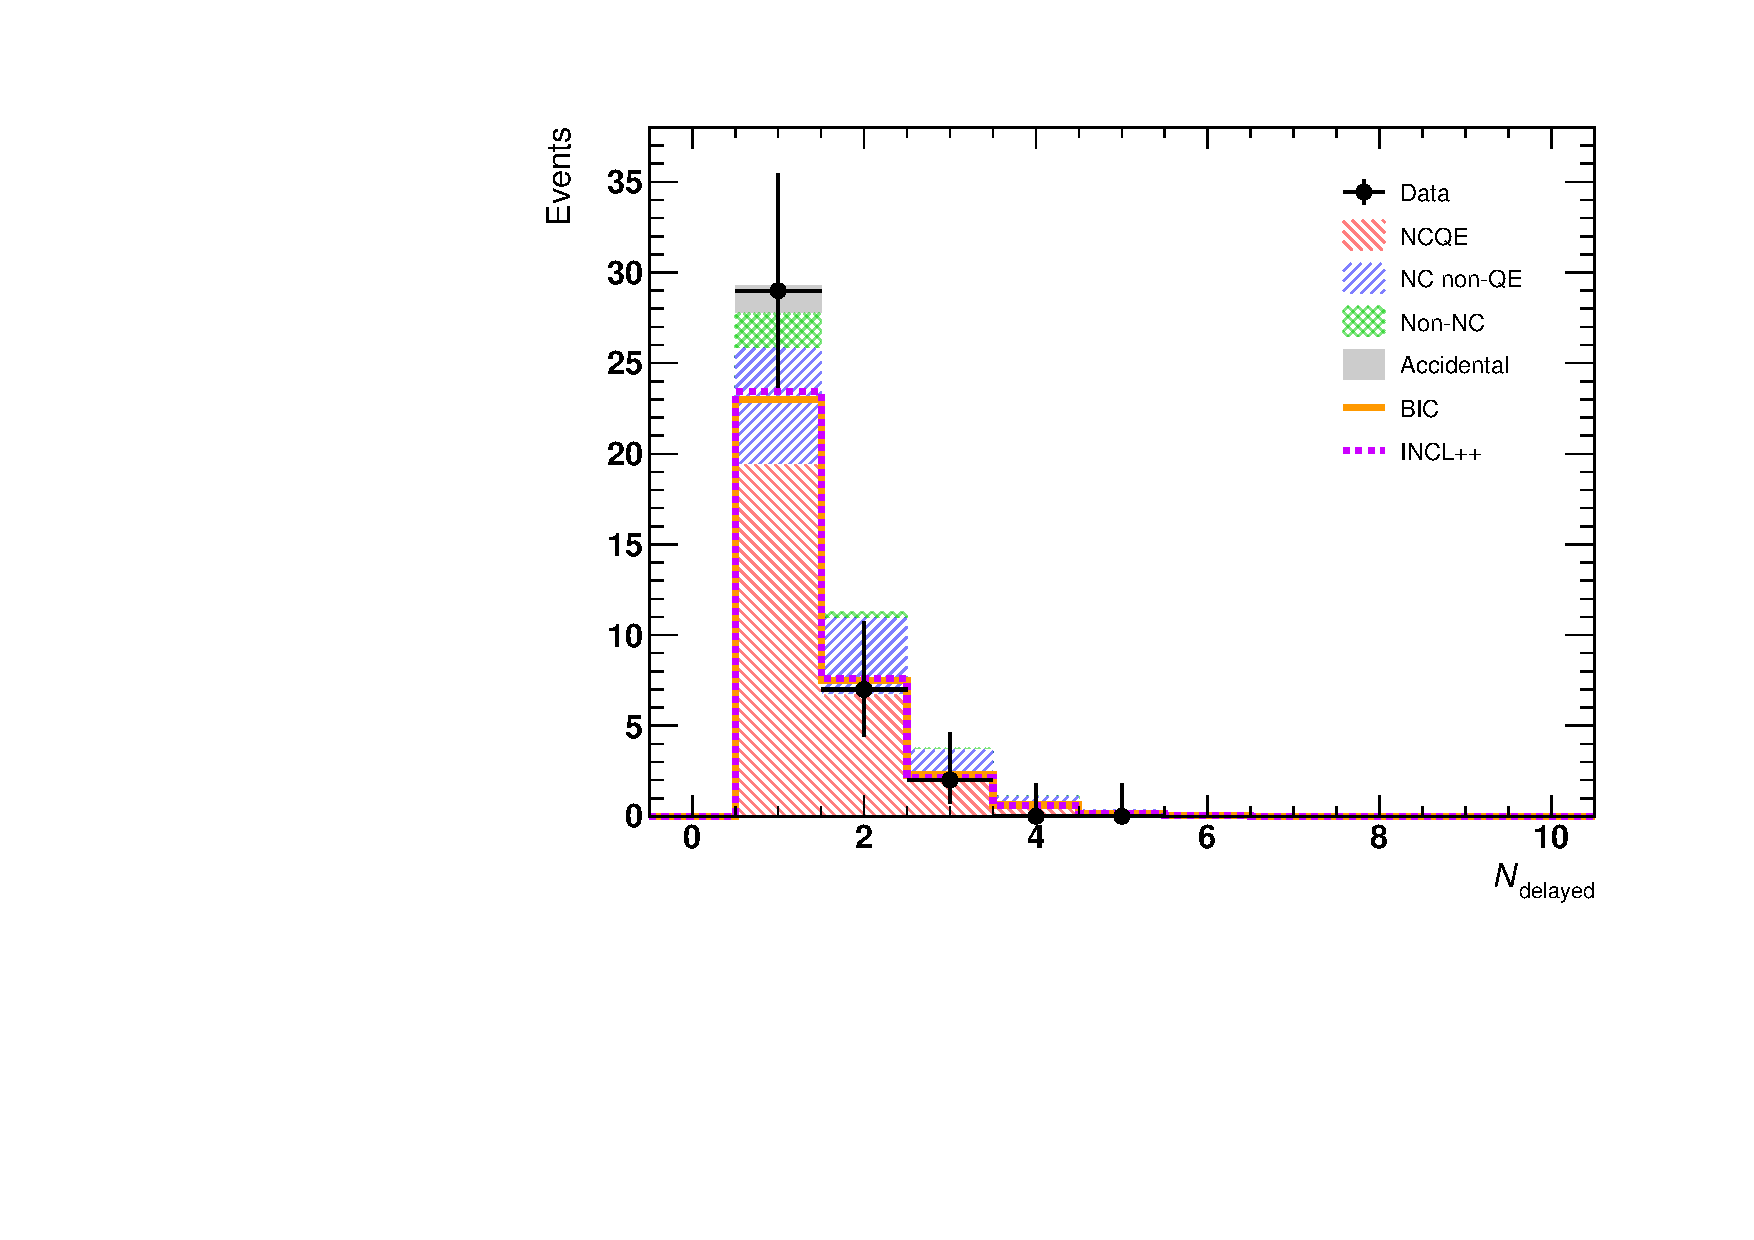
\includegraphics[width=12cm]{PDF/Figure04/Comparison/Figure04_Poisson}
%	\caption[$N_{\rm delayed}$ distribution]{
%	$N_{\rm delayed}$ distribution.
%	Each color-filled histogram shows the expected events in BERT.
%	Non-NC includes CC, spallation, and reactor neutrino events.
%	Solid and dashed line show the total expected events in BIC and INCL++, respectively.
%	In this distribution, $\theta_{\rm C}$ is greater than 50~degrees and $E_{\rm vis}$ is between 7.49~MeV and 29.49~MeV.
%	}\label{Comparison_Figure04_Poisson}
%\end{figure}

\begin{figure}[b]
	\centering
	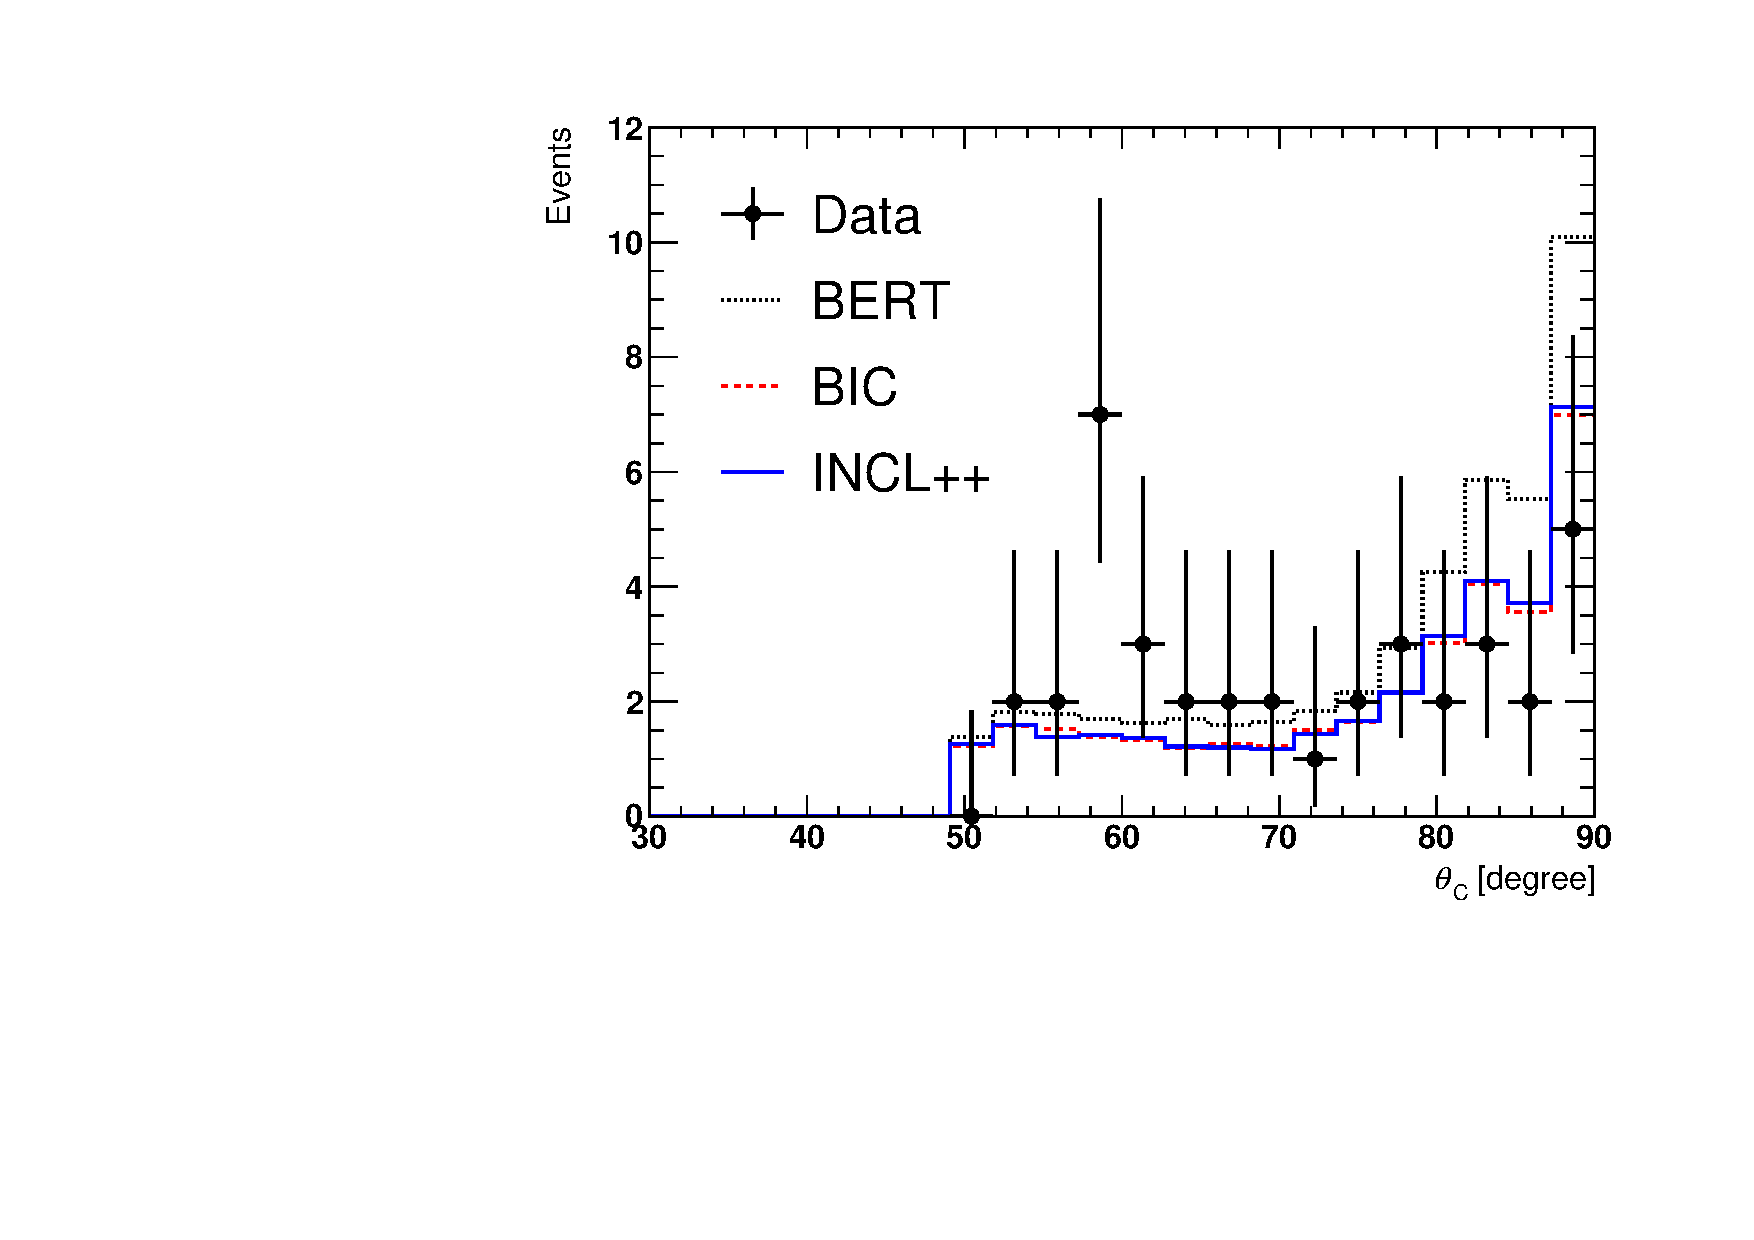
\includegraphics[width=12cm]{PDF/Figure02_02/Comparison_02/Figure02_Poisson}
	\caption[$\theta_{\rm C}$ distribution]{
	$\theta_{\rm C}$ distribution.
	Dotted, dashed, and solid line show the total expected events in BERT, BIC, and INCL++, respectively.
	In BERT, the total expected events in this distribution are the same as that in Figure~\ref{FTFP_BERT_HP_Figure02_Poisson}.
	In this distribution, $E_{\rm vis}$ is between 7.49~MeV and 29.49~MeV and $N_{\rm delayed}$ is greater or equal to one.
	}\label{Comparison_Figure02_Poisson}
\end{figure}

\begin{figure}[b]
	\centering
	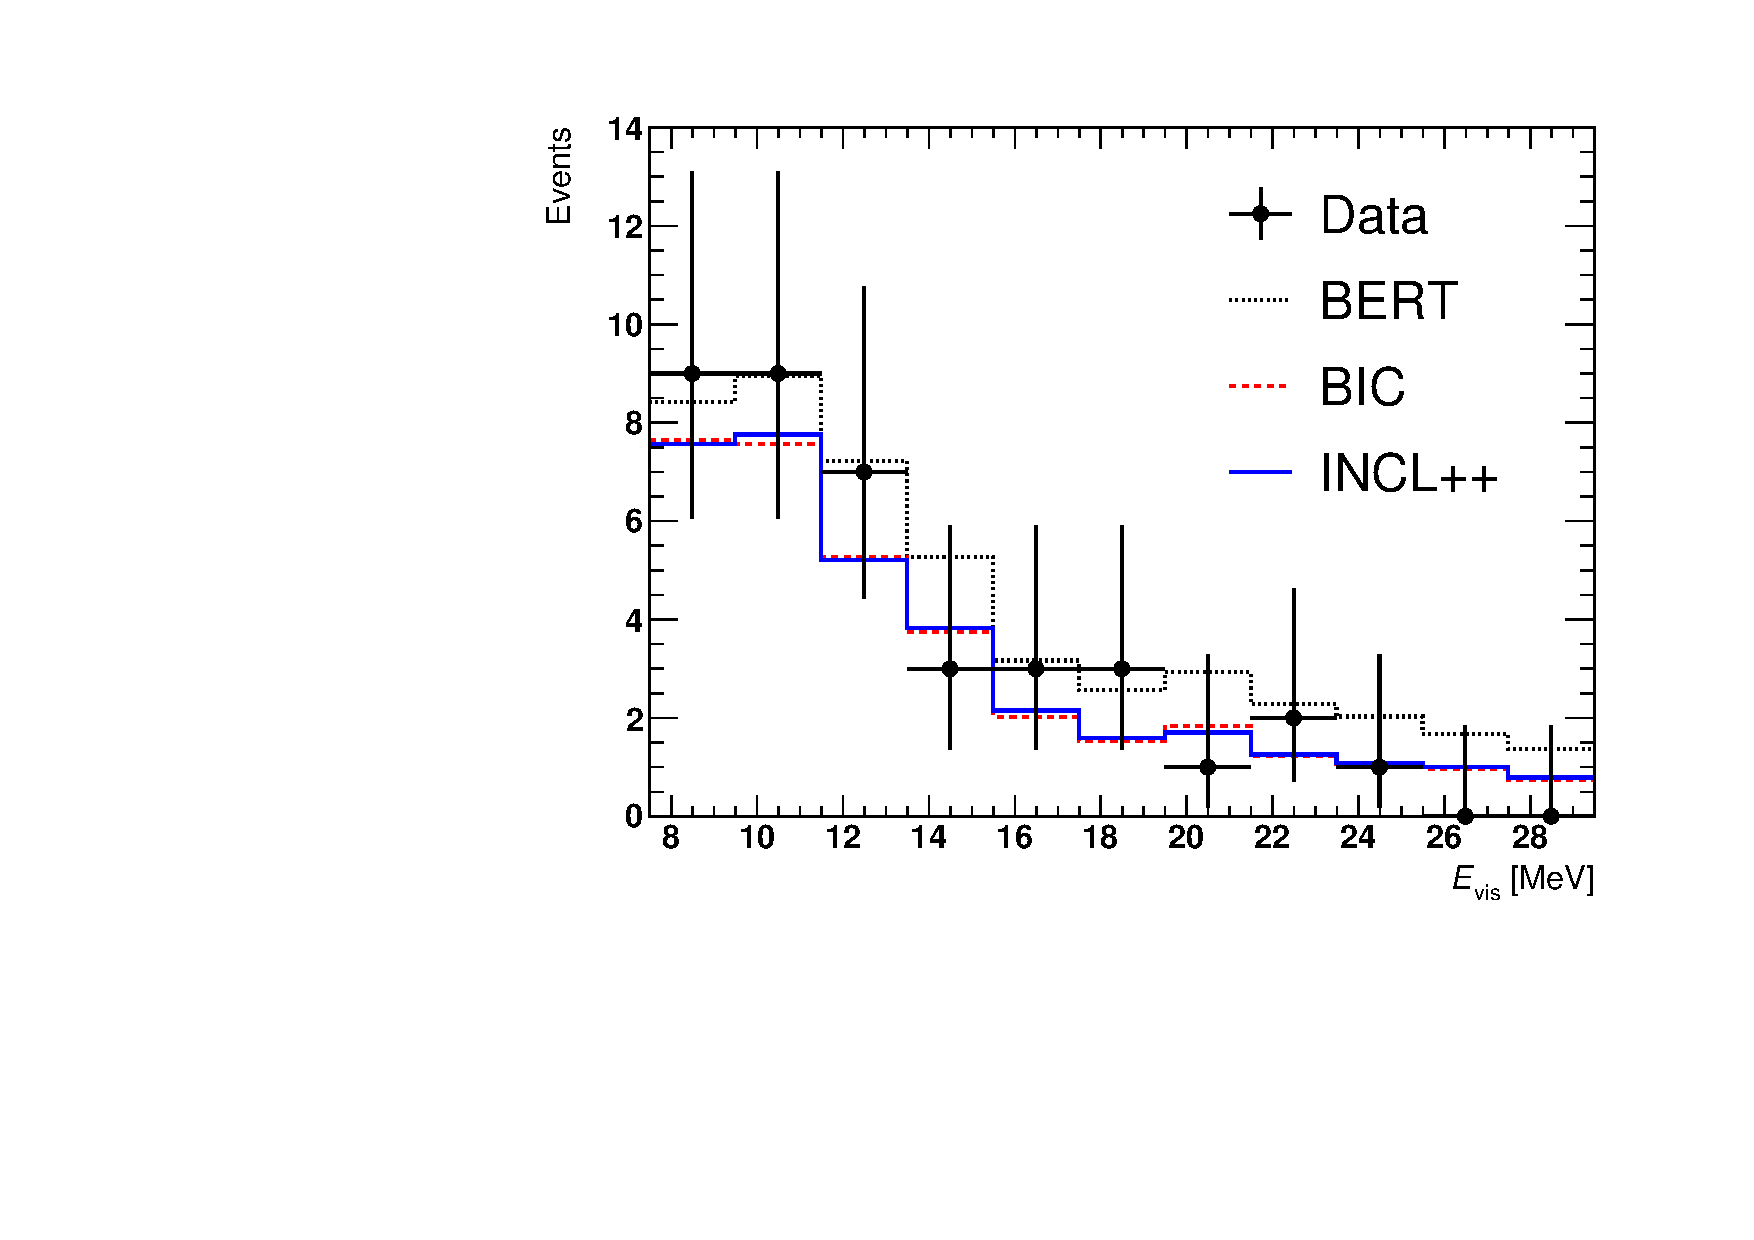
\includegraphics[width=12cm]{PDF/Figure08/Comparison_02/Figure08_Poisson}
	\caption[$E_{\rm vis}$ distribution]{
	$E_{\rm vis}$ distribution.
	Dotted, dashed, and solid line show the total expected events in BERT, BIC, and INCL++, respectively.
	In BERT, the total expected events in this distribution are the same as that in Figure~\ref{FTFP_BERT_HP_Figure08_Poisson}.
	In this distribution, $\theta_{\rm C}$ is greater than 50~degrees and $N_{\rm delayed}$ is greater or equal to one.
	}\label{Comparison_Figure08_Poisson}
\end{figure}

\begin{figure}[b]
	\centering
	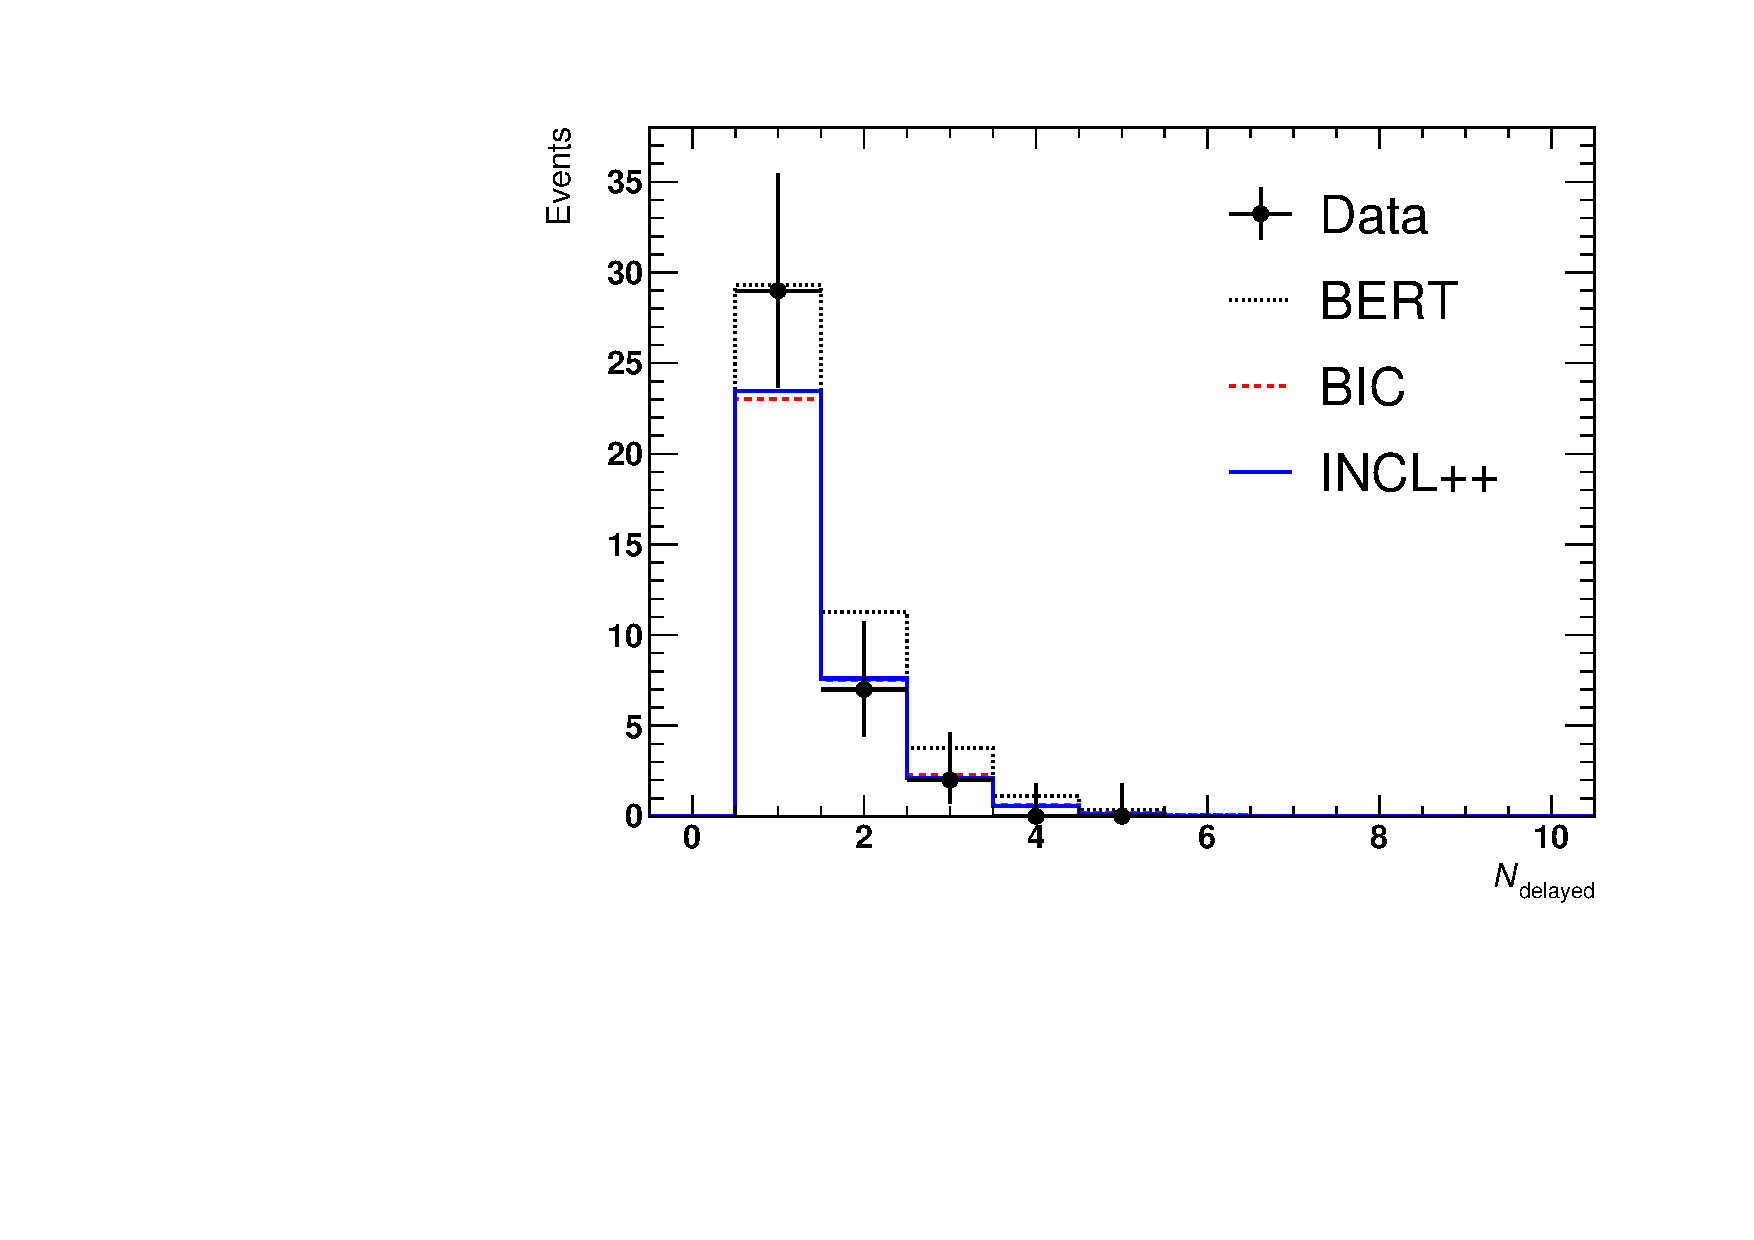
\includegraphics[width=12cm]{PDF/Figure04/Comparison_02/Figure04_Poisson}
	\caption[$N_{\rm delayed}$ distribution]{
	$N_{\rm delayed}$ distribution.
	Dotted, dashed, and solid line show the total expected events in BERT, BIC, and INCL++, respectively.
	In BERT, the total expected events in this distribution are the same as that in Figure~\ref{FTFP_BERT_HP_Figure04_Poisson}.
	In this distribution, $\theta_{\rm C}$ is greater than 50~degrees and $E_{\rm vis}$ is between 7.49~MeV and 29.49~MeV.
	}\label{Comparison_Figure04_Poisson}
\end{figure}

\hs
We calculated the chi-square $\chi^{2}$ for $\theta_{\rm C}$, $E_{\rm vis}$, and $N_{\rm delayed}$ distributions by using the Poisson-likelihood~\cite{2020Ji}.
Here, $\chi^{2}$ is defined as
\begin{eqnarray}\label{eq:chi-square}
	\chi^{2}=2\sum_{i=1}^{\rm bin} \Biggl(N^{{\rm exp},i} - N^{{\rm obs},i} + N^{{\rm obs},i}\,{\rm ln}{N^{{\rm obs},i} \over N^{{\rm exp},i}}\Biggr),
\end{eqnarray}
where ${\rm bin}$ is the number of bins, $N^{{\rm obs},i}$ is the observed number of events of $i$-th bin and $N^{{\rm exp},i}$ is the expected number of events of $i$-th bin.
The derivation of Equation~(\ref{eq:chi-square}) is summarized in Appendix~\ref{App_likelihood}.
The values of the chi-square for $\theta_{\rm C}$, $E_{\rm vis}$, and $N_{\rm delayed}$ distributions are summarized in Table~\ref{tab:chi-square}.
Due to the small statistics, the chi-square cannot give conclusive results; however, the values are smaller for BIC and INCL++ than for BERT in all distributions.

\begin{table}[h]
	\centering
	\caption[Values of the chi-square for $\theta_{\rm C}$, $E_{\rm vis}$, and $N_{\rm delayed}$ distributions]{
	Values of the chi-square for $\theta_{\rm C}$, $E_{\rm vis}$, and $N_{\rm delayed}$ distributions.
	}\label{tab:chi-square}
	\vs
	\begin{tabular}{cccc} \hline \hline
		Model        & $\chi^{2}/{\rm ndf}$ ($\theta_{\rm C}$) & $\chi^{2}/{\rm ndf}$ ($E_{\rm vis}$) & $\chi^{2}/{\rm ndf}$ ($N_{\rm delayed}$) \\ \hline
		BERT         & 23.0 / 15                               & 9.8 / 11                             & 5.8 / 5                                  \\
		BIC          & 19.6 / 15                               & 6.9 / 11                             & 3.1 / 5                                  \\
		INCL++       & 19.8 / 15                               & 6.8 / 11                             & 2.8 / 5                                  \\ \hline \hline
	\end{tabular}
\end{table}

\hs
As described in Section~\ref{Subsec_MeasurementsNCQE}, an accelerator neutrino-oxygen NCQE cross section measurement was conducted as part of the T2K experiment~\cite{2019Abe}.
The observed and expected number of events in $\theta_{\rm C}\in$ [78, 90]~degrees and $E_{\rm vis}\in$ [7.49, 29.49]~MeV obtained in the T2K data analysis are shown in Table~\ref{tab:obsexp}.
As shown in Figure~\ref{Comparison_Figure02_Poisson}, the difference between models is especially large in $\theta_{\rm C}\in$ [78, 90]~degrees.
Therefore, using the same criteria of $\theta_{\rm C}$ and $E_{\rm vis}$, we have also performed an analysis of secondary interaction model comparison using atmospheric neutrinos.
The results are also summarized in Table~\ref{tab:obsexp}.
With these selection criteria, the expected number of events in BERT is larger than the observed number of events.
The similar discrepancy was observed in T2K because the secondary interaction model is based on BERT~\cite{2019Abe,1970Coleman}.
In both cases, the differences of the expected and observed number of events in BERT are larger than that in BIC and INCL++, which shows similar trend as above.

\begin{table}[h]
	\centering
	\caption[The observed and expected number of events in $\theta_{\rm C}\in$ \lbrack 78, 90\rbrack~degrees and $E_{\rm vis}\in$ \lbrack 7.49, 29.49\rbrack~MeV in this study and T2K]{
	The observed and expected number of events in $\theta_{\rm C}\in$ [78, 90]~degrees and $E_{\rm vis}\in$ [7.49, 29.49]~MeV in this study and T2K~\cite{2019Abe}.
	In T2K, $N_{\rm delayed}$ (greater or equal to one) cut is not applied.
	}\label{tab:obsexp}
	\vs
	\begin{tabular}{lrrr} \hline \hline
		           & Model  & Expected & Observed \\ \hline
		           & BERT   & 26.8     &          \\
		This study & BIC    & 18.4     & 14       \\
		           & INCL++ & 18.9     &          \\ \hline
		T2K        & BERT   & 100.8    & 61       \\ \hline \hline
	\end{tabular}
\end{table}





\newpage

